\documentclass[11pt]{report}
\usepackage[left=1in,top=1in,right=1in,bottom=1in]{geometry} % see geometry.pdf on how to lay out the page. There's lots.
\geometry{letterpaper} % or letter or a5paper or ... etc
\pagestyle{headings}
\usepackage{geometry}
\usepackage{graphicx}
\usepackage[usenames]{color}
\definecolor{purple}{rgb}{.5, 0, .5}
\usepackage{longtable}
\usepackage{multirow} % we're not actually using these...
\usepackage{multicol}
\usepackage{verbatim} % for comment blocks
\usepackage{natbib}
\usepackage{datetime} % To set the document dates automagically
\usepackage[hidelinks]{hyperref} % for real url support in the pdf

\newcommand{\plcat}[1]{\textsf{#1}}
\newcommand{\ti}[1]{\textit{#1}}
%\newcommand{\TABx}{\textsc{Tabari}}
%\newcommand{\KEDS}{\textsc{Keds }}
\newcommand{\txt}[1]{\texttt{#1}}
% Replace with hyperef above
% \newcommand{\url}[1]{\small{\mbox{\texttt{#1}}}\normalsize} % URLs
\newcommand{\fn}[1]{\footnote{#1}} 
\newdateformat{monthyeardate}{%
  \monthname[\THEMONTH] \THEYEAR}
    
\begin{document}

\pagenumbering{gobble}

\vspace{-10pt}  

      \begin{center}
            {\Huge \bfseries PLOVER\ }\\[2ex] 
            {\LARGE Political Language Ontology for Verifiable Event Records\\ [2ex]Event, Actor and Data Interchange Specification}\\[10ex] 
            {\LARGE Open Event Data Alliance} \\[2ex] 
            {\Large \url{http://openeventdata.org/} }\\[2ex] 
%             {\Large \texttt{http://openeventdata.org/ploverdata/} }\\[6ex]            
            {\Large \url{http://ploverdata.org/} }\\[6ex]            
            {\LARGE DRAFT Version: 0.6b2\\ [2EX]\monthyeardate\today}
        \end{center}


\begin{figure}[h!]
\centering
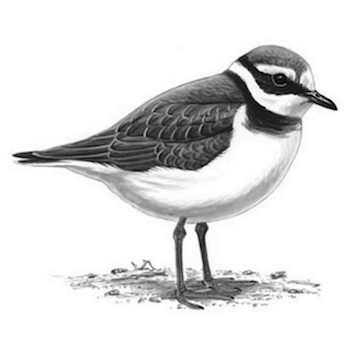
\includegraphics[width=0.40\textwidth]{media/plover_icon}
\end{figure}

\vspace{20pt}   


\begin{figure}[h!]
\centering
\includegraphics[width=0.6\textwidth]{media/cc_license}
\end{figure}





%\pagenumbering{roman}
%\tableofcontents
%\setcounter{tocdepth}{3}
%\listoftables

\chapter*{Acknowledgments}

\noindent Contributors to the development of PLOVER include, in alphabetical order, Benjamin Bagozzi, John Beieler, Liz Boschee, Patrick T.~Brandt, Andrew Halterman, Jill Irvine, Jennifer S.~Holmes, Javier Osorio and Philip Schrodt.\\

\noindent The Open Event Data Alliance is an educational and open research corporation chartered in the Commonwealth of Virginia, United States.\\

\noindent The PLOVER logo is based on a drawing found at\\ \url{http://www.rspb.org.uk/discoverandenjoynature/discoverandlearn/birdguide/name/r/ringedplover/}\\

\noindent Funding for PLOVER has been provided in part by the U. S. National Science Foundation award SBE-1539302, ``RIDIR: Modernizing Political Event Data for Big Data Social Science Research''\\

\noindent Any opinions, findings, conclusions or recommendations in this document are [only \textit{probably} still] those of [at least one of] the authors and do not necessarily reflect the views of the National Science Foundation, or any company or government agency employing or funding the authors or otherwise contributing to the document.\\

\noindent This work is licensed under a Creative Commons Attribution-ShareAlike 4.0 International License.\\

\noindent  Copyright \copyright ~2016 by the Open Event Data Alliance \\

\noindent Latest update: \today~(UTC)

\chapter{Introduction}

Event data in political science is a structured way of recording interactions
between political actors described in text. For instance, a researcher
encountering the sentence 

\begin{quotation}
A town in western Sudan's South Kordofan state has been recaptured by Sudanese
government forces from the rebel Sudan People's Liberation Army (SPLA).

(AFP\_ENG\_19970408.0772)
\end{quotation}

might want to represent it as ACTOR = ``Sudanese military", EVENT = ``capture
territory", TARGET = ``SPLA", a process that can be applied over hundreds of
thousands of reports to create datasets of thousands of such events for
answering research questions.

The software to extract and categorize these events exists (see OEDA's
Petrarch2 (\url{https://github.com/openeventdata/petrarch2}), for instance), but all
event data systems require an ontology defining what actors and events will be
recorded and how they will be defined.

Ontologies face difficult tradeoffs: broader groupings of event types and
actors are easier to define and implement, are easier to work with, and provide
data at a useful level of aggregation, especially analyzed globally. More
specialized and specific ontologies will sometimes be necessary for answering
certain research questions and allow more granular and subnational study, but
are more difficult to implement and may provide distinctions that are not
useful to most researchers. In the example above, should the event be
categorized as a general ``seize" event? Or a more specific "capture territory"?
Should the target be coded as a general "Sudanese rebel" or the very specific
``SPLA"? 

The best level of detail will depend on the question and resources of the
researcher.  PLOVER is a new event data ontology that choses to be more
general, easier to implement (including across languages), easier to use, and at the level of
detail demanded by most existing users of event data. At the same time, PLOVER
defines and provides guidance on making ``PLOVER-compliant extensions" that will
fit into the ecosystem of tools for creating and analyzing PLOVER event data.

\section{Overview}

This manual starts with a history of PLOVER and event data for users coming from CAMEO. It then defines the top-level event types that base PLOVER defines. Along with these, it describes the ``mode'' and ``context'' fields that PLOVER uses to provide more information about the event and the circumstances in which it's occuring. Next, the manual defines codes for the actors. It then lists the standard fields in a PLOVER event record before describing ``PLOVER-complient'' extensions that researchers can use for building custom datasets.

\section{History of \textsc{PLOVER}}
\pagenumbering{arabic}

During the twentieth century, two coding frameworks dominated event data research: Charles McClelland's WEIS \citep{McClelland67,McClelland76}  and the Conflict and Peace Data Bank (COPDAB) developed by Edward Azar \citep{AzarSloan75, Azar80, Azar82}. Both were created during the Cold War and assumed a ``Westphalian-Clausewitzian'' political world in which sovereign states reacted to each other primarily through official diplomacy
and military threats. While innovative when first created, these coding systems were less than optimal for dealing with contemporary issues such as ethnic conflict, low-intensity violence, organized criminal activity, and multilateral intervention. Furthermore, \citet[pg. 177]{McClelland83} viewed WEIS as only a ``first phase''; he certainly did not anticipate that it would continue to be used, with only minor modifications, for four decades. Event coding ontologies, it seems, tend to be rather sticky.

During the early 2000s, the CAMEO framework---Conflict and Mediation Event Observations---was developed,\footnote{The canonical citation for CAMEO is \cite{SGY09}, and the most recent version of the manual is found at \texttt{http://eventdata.parusanalytics.com/data.dir/cameo.html}.  The original event framework was very much the work of Deborah Gerner and \"Om\"ur Yilmaz, with contributions by various coders in the Kansas Event Data System project. The CAMEO manual contains an extended discussion of the issues considered in transitioning from WEIS to CAMEO. Additional details on the development of the automated coding underlying CAMEO can be found in \cite{Schrodt06TPM} or \texttt{http://eventdata.parusanalytics.com/utilities.dir/KEDS.History.0611.pdf}. } and originally was intended merely to support an NSF-funded project on the study of inter-state conflict mediation. Instead, it was gradually adopted as a ``next generation'' coding scheme, notably for the DARPA-funded Integrated Conflict Early Warning System (ICEWS) project \citep{OBrien10} because it corrected some of the long-recognized ambiguities in WEIS and COPDAB, and was explicitly designed both for automated coding and for the detailed coding of sub-state actors. 

As event data came into wider use in the 2010s, several problems with the CAMEO standard---which had never been intended to be a ``standard'' in the first place---became apparent. These included

\begin{itemize}
\item Almost all applications of CAMEO event data aggregated to either the 2-digit ``cue category'' or the even more general ``quad category.''\fn{Verbal cooperation, material cooperation, verbal conflict, and material conflict, with these usually defined exclusively using the 2-digit categories.} No one used all 260 codes.
\item Nonetheless, users unfamiliar with the data generating process for automated event coding sometimes assumed every code had been equally well implemented.
\item The complexity of CAMEO made it almost impossible to generate a comprehensive set of ``gold standard records'' and human coders had difficulty agreeing on how to consistently distinguish many of the subcategories: this became particularly apparent as efforts were made to implement CAMEO in Spanish and Arabic.
\item Newer coding systems provided information such as geolocation and named-entity extraction beyond the original date-source-target-event format and there was no standard for how to include these in the data.
\item The continuing emphasis on coding substate activities demonstrated the need for either new categories or contexts to deal, for example, with criminal activity and events such as natural disaster, elections, and parliamentary behavior.
\end{itemize}

Predictably, because of these and other issues, by 2015 CAMEO was beginning to ``fork'': both the ICEWS data implementing CAMEO in the BBN/Raytheon \txt{ACCENT} coder \\ (\url{https://dataverse.harvard.edu/dataverse/icews}) and the Phoenix data implementing it using the Open Event Data Alliance (OEDA) \txt{PETRARCH-2} coder  (\url{http://phoenixdata.org/}) differed significantly in some of the CAMEO categories compared to the original implementation in the University of Kansas \txt{TABARI} coder. 

To address these concerns, an informal group of academic, government and private sector producers and users of event data met and circulated drafts during the fall of 2016 to develop a new, simplified and more flexible event data specification to replace CAMEO: the end product of those deliberations is the document you are reading. The major changes are the following

\begin{itemize}
\item CAMEO's numeric categories demanded a high degree of fluency from users (e.g. remebering that that ``09'' is ``Investigate'' and ``08'' is ``Yield''). The numeric categories also implied an ordinal scale that was not always approprate: ``assault'' is more extreme than ``coerce'', but ``investigate'' isn't a more intense than ``yield''). PLOVER does away with numeric codes to solve both of these problems and instead uses only a text name for each event type.
\item A set of standardized names (``fields'') are specified for both the core event data fields and for extended information such as geolocation and extracted texts; most of these fields are optional and where available we use existing specifications, for example the \url{http://geonames.org} geographical location field names, ISO-3166 country identifiers and ISO-8601 date and time formats, and \textit{Social Conflict Analysis Database} (SCAD) protest contexts. To accomodate this flexibility, PLOVER defines events in a JSON document structure rather than the CSV formats that most social science datasets are available in. A PLOVER R package will make it easier for researchers to work with the PLOVER dataset and custom datasets using the PLOVER ontology.
\item Only the 2-digit event ``cue categories'' have been retained from CAMEO: our hope is that these are sufficiently broad and distinct that one can achieve a reasonably high level of human inter-coder agreement---hence ``verifiable''---on the coding categories, and that these distinctions can be consistently implemented, across all categories, in the automated system. These are defined in greater detail than they were in WEIS and CAMEO.
\item The CAMEO 01 and 02 categories dealing with comments have been eliminated.\fn{Ironically, this reverses a decision McClelland belatedly made---and later regretted---in the WEIS specification in the 1960s.}
\item The CAMEO 08 ``YIELD'' category has been split into verbal (\plcat{CONCEDE}) and material (\plcat{RETREAT}) components. 
\item A new category has been added for criminal behavior.
\item Much of the detail 3- and 4-digit details is now delegated to an optional $mode$ field (as well as $context$): see Section \ref{ssec:ecm} for further discussion of this.  \item A ``context'' field is available, along with standard values, to handle contexts such as disease, natural disaster, elections, parliamentary processes and cyber-security.\fn{In contrast to the Integrated Data for Events Analysis (IDEA) \cite{BBOJT03} system which was in use in the early 2000s, we are not treating disease and disaster as events with targets, instead they are a context within which other activity occurs. This, interestingly, echoes an approach used in COPDAB but not retained by WEIS and CAMEO.}
\item The complexity of substate actor codes has been limited, and the allowable substate modifiers have been substantially simplified. 
\item Standard optional fields have been defined for some categories, and the ``target'' is optional in some categories.
\item We have converted all of the examples in the CAMEO manual to an initial set of English-language ``gold standard records'' for validation purposes---these files can be found at\\ \url{https://github.com/openeventdata/PLOVER/blob/master/PLOVER_GSR_CAMEO.txt}---and we expect to both expand this corpus and extend it to  at least Spanish and Arabic cases. This documentation includes the English-language gold standard records from the CAMEO manual.
\end{itemize}

Because PLOVER is generally a simplification of CAMEO---the new \textsf{CRIME} category is the one exception---our expectation is that it will be relatively easy to transition the existing CAMEO-based coders into this by simply collapsing the two- and three-digit categories; a similar simple recoding will allow older CAMEO-coded data sets to be converted to their PLOVER equivalents. The standardization of the JSON field names---as well as adoption of JSON as the data interchange format---will allow the development of general-purpose utilities that can work with all formats, in contrast with the current proliferation of incompatible CSV and tab-delimited formats.

\section{Issues we will not be addressing}\label{sec:nothing}

In the discussions leading to the development of PLOVER, several additional open issues were raised that we have decided to remain agnostic on:

\begin{description}
\item[Temporal markup:] This is emerging as a major issue, particular among users who are interested in the long-standing objective of automated chronology generators. While there are some significant efforts on this in the NLP community---\url{http://www.timeml.org/}---we don't feel we currently have the experience required to make recommendations.
\item[Number of events per sentence:] Everyone in the community now has a collection of sentences that could be interpreted as containing anywhere from one to a half-dozen or more events. While this is nominally an ontological issue---``the branch of metaphysics dealing with the nature of being''---the ability to resolve it will be highly dependent on specific parser/coder implementations, so we're leaving it at that level. Same for sentence-level vs paragraph- or article-level coding.
\item[De-duplication:] There is no consensus on this beyond noting that the widely-used ``one-a-day filtering'' is probably not a good idea,\fn{See \texttt{http://eventdata.parusanalytics.com/papers.dir/Schrodt.TAD-NYU.EventData.pdf}} and it is a topic where there is currently active research and experimentation, so we're leaving it alone.
\end{description}

As a more general caveat, we would very much encourage anyone who is using a PLOVER-coded data set to look carefully at the software used to implement it, particularly with regard to
\begin{itemize}
\item The motivations (and resources available) for producing the data, which will often provide information on how much attention was given to various categories. 
\item If the coder is dictionary-based, the event and actor dictionaries if these are available. If the coder is classifer-based, the training cases if these are available.
\item Recall/precision tradeoffs and how these play out across different news sources: we are not aware of any existing parser/coder that is optimal for everything from a Reuters story written and edited by people trained at Oxford to a BBC radio transcript from a static-filled French radio report out of Goma, DRC quickly translated into English by a non-native speaker of either language.
\end{itemize}

OEDA was founded on the principle that there is no ``one data set to rule them all'': different implementations will have different strengths. PLOVER is at least as much a data-interchange format as a coding ontology, and should simplify the ability of the research to check the robustness of results by looking at multiple independent coding efforts. Do it!



\section{Why ``PLOVER''?}

Plovers (\textit{Charadriidae}) are a globally-distributed family of short-billed gregarious wading birds who spend their lives frantically poking through endless stretches of sand and muck trying to find something of interest. It is difficult to imagine a better analogy to the process of coding event data.

%%%%%%%%%%%%%%%%%%%%%%%%%%%%%%%%%%%%%%%%%%%%%%%%%%%%

\chapter{Event Categories}

\textbf{General observation (pas 2016-10-19):} I've included separate $mode$ and/or $context$ lists for \plcat{CONSULT, MOBILIZE, CRIME, COERCE, PROTEST} and \plcat{ASSAULT} but in fact we could probably usefully include them for almost all of the categories. In contrast to CAMEO, these are optional, but they do provide a systematic way of providing more detail. However, there is still too much detail specific to mediation in here.

\section{Event, Mode, and Context}\label{ssec:ecm}

As noted above, most\fn{``most'' because some of the details coded in CAMEO, particularly those dealing specifically with mediation, have been eliminated.} of the detail found in the 3- and 4-digit categories of CAMEO is now found in the $mode$ and  $context$ fields in PLOVER. More generally, PLOVER takes the general purpose ``events'' of CAMEO (as well as the earlier WEIS, IDEA and COPDAB ontologies) and splits these into three components: generally ``$event-mode-context$'' corresponds to ``$what-how-why$.'' We anticipate at least four advantages to this
\begin{enumerate}
\item The three ``$what-how-why$''components are now distinct, whereas various CAMEO subcategories inconsistently used the $how$ and $why$ to distinguish between subcategories.
\item We are probably increasing the ability of classifiers---as distinct from parser/coders---to assign $mode$ and $context$ compared to their ability to assign subcategories.
\item In initial experiments, it appears that the  approach \textit{much} easier for humans to code than the hierarchical structure of CAMEO because a human coder can hold most of the relevant categories working memory (well, that and a few tables easily displayed on a screen)\footnote{PLOVER coding may also be easier because everything in the $event-mode-context$ coding uses words, not numerical codes, so coders will probably be using the parts of the brain (Broca's area) which are specialized for processing words. No known specialized cognitive facility exists for handling some 250 2-to-4-digit codes.}
\item Because the words used in differentiate $mode$ and $context$ are generally very basic, translations of the coding protocols into languages other than English is likely to be easier than translating the subcategory descriptions found in CAMEO. 
\end{enumerate}

While both $mode$ and $context$ will usually take a single value, in some instances multiple values will be appropriate and this is allowed (and preferable to generating multiple events from a single text). Both fields are optional, and unless an ``other'' category is explicitly specified---this has been provided in a couple of the event categories to provide compatibility with other coding systems---if no existing values seem appropriate, the field should be left null, though perhaps with some details provided in the $comment$ field, particularly when the record is generated using human coding.

In general, verbal activities only have a $context$ since their $mode$ is just ``verbal.'' The exceptions are \plcat{CONSULT} where the $mode$ indicates how the consultation was done, and \plcat{THREATEN} where the $mode$ indicates what action is being threatened. 

We anticipate that in general---and consistent with earlier event coding schemes---it will be possible to code $mode$ from the same sentence used to code the event. $context$, in contrast, will often need to be coded at the paragraph- or document-level: this differs from earlier automated coding, though probably is similar to human-coded data such as COPDAB and BCOW where $context$-like fields were coded.


\section{AGREE}

Agree to, offer, promise, or otherwise indicate willingness or commitment to cooperate.  All cooperative actions reported in future tense are also taken to imply intentions. 

\subsection{Requires target: No}

\subsection{Supplementary fields: None}

\bigskip  

\section{CONSULT}

All consultations and meetings: this includes visiting and hosting visits, as well as meeting at a neutral location, and consultation by phone or other media. Other useful keywords: ``Holding talks'' and ``discussions'', ``negotiations, bargaining, or discussions''. See the discussion in Section \ref{sec:recip} on the treatment of actors in \plcat{CONSULT} events.

\subsection{Requires target: No}

\plcat{CONSULT} events where there is no clear distinction between whether an actor is hosting or visiting, all participants are coded as source actors. 

\subsection{Supplementary fields: }

\begin{table}[htp]
\caption{CONSULT modes}
\begin{center}
\begin{tabular}{|l|p{13cm}|}
\hline
Name & Content \\
\hline
host & Meeting is hosted by source\\
visit & Meeting is hosted by target \\
third-party & Meeting is hosted by a third party\\
multilateral & Meeting occurs in a multilateral context, typically an alliance or IGO\\
phone & Consultation occurs via phone or some other remote medium\\
\hline
\end{tabular}
\end{center}
\label{tab:consultmode}
Adapted from CAMEO.
\end{table}%

\newpage

\section{SUPPORT}

Initiate, resume, improve, or expand diplomatic, non-material cooperation; express support for, commend, approve policy, action, or actor. This event form is a verbal act. Use this code only for political, diplomatic, and non-material support, including recognition of newly independent states, new governments that might have come to power through unconventional means, and initiation of diplomatic ties with an entity for the first time, as are actions which ratify, sign, or finalize an agreement or treaty.
 
\subsection{Requires target: No}

\subsection{Potential ambiguities}

\begin{itemize}
\item Formal pardons and amnesties of arrested persons should be coded as \plcat{CONCEDE}; the actual release  or exchange of prisoners should be coded as \plcat{RETREAT}.

\item Expressions of regret or remorse for an action or situation should be coded as \plcat{CONCEDE}.

\item Promises to sign or ratify agreements and treaties are coded as \plcat{AGREE}

\item Military cooperation or defense should be coded as \plcat{COOPERATE} with a \txt{military} $context.$
\end{itemize}

\subsection{Supplementary fields: None}

\newpage

\section{CONCEDE}

This covers verbal concessions which have no immediate material consequences, including promised of future concessions, including easing of administrative or legal restrictions on persons and organizations, remove curfews, suspending protests, declarations (but not implementations) of ceasefires and withdrawals from territory.

\plcat{CONCEDE}, like the verbal components CAMEO/WEIS predecessor \plcat{YIELD}, is inherently problem since many concessions deal with promises that certain things will \ti{not} happen, or will happen in the distant future (e.g. many policy changes). So, for example, the lifting of a curfew is, effectively, a promise that people will not be arrested for violating the curfew, which itself is not an event. We're treating such concessions as verbal rather than material even though sometimes they have material consequences, e.g. people coming out in the streets after a curfew is lifted. But only if they believe the government. As noted in Section \ref{sec:nothing}, PLOVER isn't really set up to deal with these levels of event dependence. 

\begin{comment}

pas 2006-10-20

I split CAMEO YIELD but and most of the old categories break out pretty easily but I'm still not quite sure the following belongs here

\item Yield by relinquishing political power, either via voluntary concessions or involuntary surrenders. Use this code when source surrenders power after being challenged through legitimate institutional channels (e.g. elections) or other coercive strategies (e.g. military coups). The target can either be the challenger(s) or the country as a whole.

ptb 2016-12-20
How does this interaction with the hex codings of negative events in PETR 2?

\end{comment}

\subsection{Requires target: No}

\subsection{Supplementary fields: Use at least a few of the CAMEO cases?}


\bigskip
%\newpage  

\section{COOPERATE}

Initiate, resume, improve, or expand \ti{mutual} material cooperation or exchange, including

\begin{itemize}
\item Initiate, resume, improve, or expand economic exchange or cooperation.

\item Military exchanges such as joint military games and maneuvers.

\item Cooperation on judicial matters, such as extraditions and war crimes.

\item Voluntary exchanges or sharing of intelligence and other significant information .

\end{itemize}

\noindent \plcat{COOPERATE} is distinguished from \plcat{AID} because the activity is generally understood to directly benefit both parties, whereas  \plcat{AID} is understood to primarily benefit only the recipient. 

\subsection{Requires target: Yes}

\subsection{Supplementary fields: None? Or rely on the general context codes?}


\newpage

\section{AID}

All provisions of providing material aid whose material benefits primarily accrue to the recipient. Examples include: 

\begin{itemize}

\item Monetary aid and financial guarantees, grants, gifts and credit.

\item Military and police assistance including arms and personnel.

\item Humanitarian aid such as emergency assistance.

\item Asylum, both to persons in its territories (territorial asylum) and diplomatic asylum on the premises of an embassy.

\end{itemize}

\subsection{Requires target: Yes}

\subsection{Supplementary fields: None? Or capture the monetary, manpower, and magnitudes from the context?}


\bigskip  


\section{RETREAT}

\plcat{RETREAT} covers any events---not just military ``retreat'' from territory---which have an immediate (not simply promised) material consequences, such as the release of prisoners and hostages, repatriation of refugees, the return of  confiscated property, allowing the entry of observers, peacekeepers, or humanitarian workers, disarming, observing a ceasefire or otherwise ending active conflicts, and, of course, a military retreat from, or ceding, territory. \plcat{RETREAT} also covers resignations of government officials.

\subsection{Requires target: No}

\subsection{Supplementary fields: Almost certainly need some}


\bigskip  


\section{INVESTIGATE}

All investigations, including those of historical cases. Examples include investigations of  criminal activity (theft, killing, etc) and corruption, human rights abuses, war crime, and violations of basic freedoms, military activities such as violations of ceasefire, seizures, and invasions.

\subsection{Requires target: No}

\subsection{Supplementary fields: None?}

\newpage  

\section{DEMAND}

All demands and orders. Demands are stronger or more forceful than a request or appeal---which is not coded in PLOVER---and potentially carry more serious repercussions, although not as much as threats. Coding will need to rely primarily on the language used by reporters to make this distinction.  All demands are verbal acts. 

Examples from the CAMEO manual include:

\begin{itemize}
\item Demand that target engages in some form of material or economic exchange or assistance.
\item Demand that target engages in or expands military relations or assistance.
\item Demand that target engages in or expands cooperation in judicial matters.
\item Demand that target exchanges intelligence or information.
\item Demand expansion of diplomatic ties or non-tangible support on particular policies.
\item Demands by refugees to be let into the territories of other countries (which should be coded as targets) and asylum demands all fit here. These are not necessarily verbal acts; refugees could be actively seeking shelter or refuge in target countries or regions.
\item Demand that the target provides military protection or peacekeeping forces  for itself or on behalf of another party.
\item Demand for elections, changes in leadership or regime, or constitutional/institutional/policy change.
\item Demand provision or expansion of social, political, or other rights, as well as demands for provision of compensation for previously violated rights.
\item Require, demand major institutional, constitutional, or regime change.
\item Demands for fundamental changes in the political system (e.g. democratization) as well as more limited institutional changes (e.g. changing electoral law).
\item Demand that target relaxes administrative restrictions.
\item Demand that target stops political protest activities.
\item Demand that target releases persons (e.g. prisoners, hostages) or property.
\item Demand that target lifts or eases economic sanctions, boycott, or embargo.
\item Demand that target allow access to international actors, such as observers, humanitarian agencies, and peacekeeping forces.
\item Demand that target stops fighting or takes measures to ease military conflict or tension, for example ceasefires, military withdrawals, and demobilization.
\item Order party(ies) to meet, negotiate; this event form can be initiated by either the adversaries or other third parties.
\item Order parties to a conflict to reach a settlement, agreement, or resolution of conflict. 
\item Demand that a third party mediates a conflict or that adversaries accept mediation of another party.
\end{itemize}


\subsection{Requires target: No}


\subsection{Potential ambiguities}

\begin{itemize}
\item This category only applies to verbal demands: demands that take the form of demonstrations, protests, etc. are coded as \plcat{PROTEST}.
\item When one or more parties to a conflict call for ending the conflict, that is taken to be an expression of intent on the part of that source actor and is thus coded as \plcat{AGREE}.

\end{itemize}

\subsection{Supplementary fields: None? -- obviously a lot of \ti{context} fodder in that list...}

\newpage  


\section{DISAPPROVE}

Express disapprovals, objections, and complaints; condemn, decry a policy or an action; criticize, defame, denigrate responsible parties.

Examples from the CAMEO manual include:

\begin{itemize}
\item  Allege, charge the target with, or blame for engaging in crime or corruption.
\item Allege, charge the target with, or blame for human rights violations, such as arbitrary detentions for prosecutions, torture, and slavery.
\item Allege, charge the target with, or blame for initiating hostilities or engaging in questionable or unjustifiable military actions such as violations of ceasefire, or with war crimes.
\item Allege, charge the target with, or blame for spying, espionage, or treason.
\item Solicit other parties to take actions against the target.
\item Written and institutionalized protests, appeals, and all petition drives and recalls. % Do we want the word protest here?
\item Sue, file civil or criminal lawsuit at domestic or international courts. Source must be the plaintiff or the state, and target must be the defendant.
\item Find guilty or liable at a court of law. Source must be the court in question, which could be domestic or international, and target must be the defendant. This event form refers typically to rulings against non-individuals, where imprisonment is not an issue. When individuals are found guilty and are therefore detained, use \plcat{COERCE} instead.

\end{itemize}

\subsection{Requires target: No}

\subsection{Supplementary fields: None?}

\newpage  


\section{REJECT}

All rejections and refusals. Examples from the CAMEO manual include:

\begin{itemize}

\item Refuse to engage in or expand material exchange. Note the difference between refusing to establish or expand material cooperation and reducing or eliminating existing ties \plcat{SANCTION}.
\item Refuse to engage in or expand economic ties.
\item Use this code for rejections of mutual economic exchange, such as trade and investment; rejection to provide financial aid (or cancel debt) is coded as CAMEO 1221 instead.
\item Refuse to engage in or expand military ties.
\item Use this code for rejections of mutual military exchange; rejection to provide military aid is coded as \plcat{SANCTION} instead.
\item Refuse to engage in or expand cooperation in judicial matters, including  extraditions or other matters pertaining to legal proceedings.
\item Refuse to engage in or expand cooperation in intelligence or information sharing.
\item Refuse to extend financial, military or humanitarian assistance. Refusals to provide shelter or refuge should also be coded here. 
\item Refuse to provide peacekeeping forces or other form of military protection;; refusals by adversaries to grant access to peacekeepers.
\item Refuse to change leadership or relinquish power.
\item Refuse to change a given policy.
\item Refuse to provide or respect social, political, economic or other rights and freedoms.
\item Refuse to make fundamental political changes, such as moving from one type of a political system to another and reforming political institutions or key laws.
\item Reject requests, refuse or decline to ease administrative sanctions, such as censorship, curfew, state of emergency, and martial law.
\item Reject requests, refuse, or decline to reduce or stop political protest activities, such as demonstrations and rallies.
\item Reject requests, refuse, or decline to release or return persons or property.
\item Reject requests, refuse, or decline to reduce or eliminate economic sanctions, boycotts, or embargoes.
\item Reject requests, refuse or decline to allow access to international actors such as observers, humanitarian agencies, and peacekeeping forces.
\item Reject requests, refuse, or decline to stop fighting or take measures to ease military conflict or tension, including ceasefires, military withdrawals, and demobilization.
\item Refuse to meet, discuss, or negotiate, including involvement of mediators or mediation initiatives.
\item Reject a proposal or request for a final, comprehensive settlement, peace proposal, or resolution.
\item Disobey, challenge, or resist laws or norms.This event category covers both civilian disobedience and official defiance.
\item Refuse to assent or formally reject legislative proposal, recommendation, or resolution.
\end{itemize}

\subsection{Requires target: No}

\subsection{Supplementary fields:}

None?---for the time being we're going to see whether everything can be done with $context$ rather than setting up $mode$ categories.

\newpage  


\section{THREATEN}

All threats, coercive or forceful warnings with serious potential repercussions. Threats are typically verbal acts. Examples from the CAMEO manual include:

\begin{itemize}

\item Threats to reduce or eliminate provision of material assistance---economic, military, humanitarian, and peacekeeping.

\item Threaten to restrict normal economic interactions by imposing sanctions, boycotts, or embargoes.

\item Threaten to reduce or formally sever ties. Non-force threats to declare independence, resign, withdraw diplomats, reduce or break diplomatic ties, etc.\ are all coded here.

\item Threaten to impose or expand non-force administrative restrictions and penalties not otherwise specified.

\item Threaten to impose or expand restrictions on fundamental freedoms, such as freedoms of speech, expression, and assembly. 
\item Threaten to ban political activities of particular parties or individuals.
\item Threatened with imprisonment or other measures of repression.

\item Threaten to enforce a deadline beyond which inhabitants of an area are not permitted to be on the streets or in public places.

\item Threaten with suspending certain given rights or the whole constitution by imposing state of emergency or military rule.

\item Threaten to mobilize or engage in actions of political dissent such as protest demonstrations, hunger strikes, strikes or boycotts, physical obstructions into buildings or areas, and riots.

\item Threaten to break-up or withdraw from discussion, negotiation, or meeting.

\item Threaten to reduce or stop international intervention by expelling or withdrawing observers, humanitarian agencies, peacekeepers, etc.

\item Threats by international agencies to withdraw their involvement as well as threats by host countries to expel such actors are coded here. 
\item Threaten dissidents with forcible subjugation.
\item Threats to imprison as well as to use force to clamp down on opposition activities are coded here. 
\item Threaten to prevent entry into and/or exit from a territory using military measures.
\item Threaten to occupy, seize control of the whole or part of a territory.  This event form is typically a verbal act and is distinct from \plcat{FIGHT}, which refers to military occupations that have been or are being carried out.
\item Threaten to use violence, including terrorist activities

\item Give a final warning, ultimate demand or order, the rejection of which carries the risk of some form of retaliation by the party issuing the ultimatum. 
\end{itemize}

\subsection{Requires target: No}

\subsection{Supplementary fields}

\begin{table}[htp]
\caption{THREATEN modes}
\begin{center}
\begin{tabular}{|l|l|}
\hline
Name & Content \\
\hline
restrict & restrict movement of people or goods, including boycotts, strikes,  \\
& blockades, and curfews \\
ban & threaten to ban political activities of particular parties or individuals \\
arrest & arrest, detain, imprison \\
relations & threaten to suspend relations, talks \\
political & ban political activities or restrictions on fundamental freedoms, \\
& such as speech, expression, and assembly\\
expel & expel diplomats, peacekeepers, NGOs \\
territory & threaten to occupy, seize control of the whole or part of a territory \\
violence & threaten violence \\

\hline
\end{tabular}
\end{center}
\label{tab:threatmode}
\end{table}%




\newpage  


\section{PROTEST}

All civilian demonstrations and other collective actions carried out as protests against the target actor: Dissent collectively, publicly show negative feelings or opinions; rally, gather to protest a policy, action, or actor(s).

\subsection{Requires target: No}

\subsection{Supplementary fields:}

\begin{description}
    \item[context:] Context (topic) of protest: see Table \ref{tab:protestcontext} 
    \item[mode:] Mode of protest: see Table \ref{tab:protestmode} 
    \item[size:]  number of participants (integer or code) 
    \item[injured:] number injured 
    \item[eventLoc:] Location of event 
\end{description}


\begin{table}[htp]
\caption{PROTEST contexts}
\begin{center}
\begin{tabular}{|l|l|}
\hline
Name & Content \\
\hline
election   &   elections\\
political   &   political and constitutional reforms\\
economic &   economy, jobs\\
food           &   food, water, subsistence\\
environment            &   environmental degradation\\
discrimination            &   ethnic discrimination, ethnic issues\\
religion           &   religious discrimination, religious issues\\
education            &   education\\
foreign            &   foreign affairs/relations\\
war            &   domestic war, violence, terrorism\\
rights             &   human rights, democracy\\
pro-govt             &   pro-government\\
assets             &   economic resources/assets\\
other             &   other\\
unknown             &   unknown, not-specified\\    
\hline
\end{tabular}
\end{center}
\label{tab:protestcontext}
\raggedright{Adapted from Salehyan and Hendix, \textit{Social Conflict Analysis Database} (SCAD)
Version 3.2: \url{https://www.strausscenter.org/images/codebooks/SCAD\_32\_Codebook.pdf}}\\~

\textbf{Observations based on coding CAMEO GSRS}
\begin{enumerate}
\item Added ``political''
\item ``ethnic'' might be a better term than ``discrimination' 
\item PTB: Do we want to compare these classifications of modes to those used by Chenoweth and MECC?
\end{enumerate}

\end{table}%

\begin{table}[htp]
\caption{PROTEST modes}
\begin{center}
\begin{tabular}{|l|p{13cm}|}
\hline
Name & Content \\
\hline
demo-org & Organized Demonstration. Distinct, continuous, and largely peaceful action directed toward
members of a distinct `other' group or government authorities.  Clear leadership or organization(s) can be identified.\\
demo-spon & Spontaneous Demonstration. Distinct, continuous, and largely peaceful action directed
toward members of a distinct `other' group or government authorities. Clear leadership or
organization cannot be identified.\\
riot-org & Organized Violent Riot. Distinct, continuous and violent action directed toward members of
a distinct `other' group or government authorities. The participants intend to cause physical injury and/or
property damage. Clear leadership or organization(s) can be identified.\\
riot-spon & Spontaneous Violent Riot. Distinct, continuous and violent action directed toward members
of a distinct `other' group or government authorities. The participants intend to cause physical injury
and/or property damage. Clear leadership or organization(s) cannot be identified.\\
strike-gen & General Strike. Members of an organization or union engage in a total abandonment of
workplaces and public facilities.\\
strike-lim & Limited Strike. Members of an organization or union engage in the abandonment of
workplaces in limited sectors or industries.\\
strike-hun & Hunger Strike (from CAMEO 142x).\\
boycott & Boycott (from CAMEO 143x).\\
obstruct & Obstruct passage (from CAMEO 144x).\\
\hline
\end{tabular}
\end{center}
\label{tab:protestmode}
\raggedright{Adapted from Salehyan and Hendix, \textit{Social Conflict Analysis Database} (SCAD)
Version 3.2: \url{https://www.strausscenter.org/images/codebooks/SCAD\_32\_Codebook.pdf}}\\~

\textbf{Observations based on coding CAMEO GSRS}
\begin{enumerate}
\item At the sentence level, it is usually not going to be possible to differentiate the ``org'' and ``spon'' status, so perhaps this should just to reduce to ``demo'' and ``riot''
\item ``ethnic'' might be a better term than ``discrimination' 
\end{enumerate}
\end{table}%

\newpage  

\section{CRIME}

\plcat{CRIME} events are non-political actions which are considered crimes in the jurisdiction where they occur: Table \ref{tab:crimemode} lists the common examples. This category is not intended for the coding of acts of civil disobedience, revolt and other activities which, while criminal from the perspective of the government, are primarily political in nature.

\subsection{Requires target: No}

\subsection{Potential ambiguities}

\begin{itemize}
\item There is often a great deal of ambiguity as to whether some activities are criminal or political: for example, confiscatory activities by a weak militarized group with little local support. Usually such distinctions will not be apparent at the sentence---or even article---level and need to be resolved elsewhere in the analysis, for example by the classification of the actor.
\end{itemize}

\subsection{Supplementary fields}

\begin{description}
    \item[mode:] Mode of crime: see Table \ref{tab:crimemode} (PTB: What is the source of these crime modes?)
    \item[size:]  any number; typically monetary amount but, for example, could be number of credit card numbers stolen 
    \item[eventLoc:] Location of event 
\end{description}


\begin{table}[htp]
\caption{CRIME modes}
\begin{center}
\begin{tabular}{|l|l|}
\hline
Name & Content \\
\hline
murder & murder \\
assault & assault \\
sex-violence & sexual violence \\
sex-work & illegal provision of sexual services for money or goods \\
theft & theft, robbery and burglary, including vehicular theft\\
kidnap & kidnapping and hijacking \\
narcotics & narcotics, including production, transport and sale \\
smuggling & smuggling (property)  \\
trafficking & smuggling/trafficking (humans)  \\
trespass & trespass; illegal mining, logging, fishing \\
arson & arson \\
vandalism & vandalism and other destruction of property \\
extortion & extortion \\
corruption & bribery and other corruption of officials \\
financial & money laundering, tax evasion, insider-trading, embezzlement \\
cyber & cyber-crime \\
war & war crimes \\
\hline
\end{tabular}
\end{center}
\label{tab:crimemode}
\end{table}%


\newpage  

\section{SANCTION}

All reductions in normal, routine, or cooperative relations not otherwise specified. Note that this is not confined to formal ``sanctions''---\plcat{SANCTION} was just the best word we could find for WEIS and CAMEO's ``REDUCE RELATIONS''

Examples from the CAMEO manual include:

\begin{itemize}
\item Curtail, decrease, break, or terminate diplomatic exchange.

\item Cancellation of meetings, withdrawal, or expulsion of diplomats and termination of other diplomatic activities 

\item Reductions or terminations of aid not otherwise specified.
\item Decrease or terminate provision of economic, military or humanitarian aid.
\item Stop or restrict commercial or other material exchange as a form of protest or punishment.
\item Terminate discussions, negotiations. Use this event form to code failed negotiations and walk-outs, as well as other disruptions of planned negotiations. Note that the termination can be either unilateral or bi/multi-lateral.
\item Terminate mediation activities.
\item Terminate the presence of groups or organizations: this covers both expulsions by host authorities and withdrawals by guest groups or organizations, as well as diplomats are withdrawn or expelled. .   \item Terminate the deployment or presence of peacekeeping forces, inspectors or other observers.
\item Terminate the presence of aid agencies or other non-governmental organizations helping civilians.
\end{itemize}

\subsection{Requires target: Yes}

\subsection{Potential ambiguities}

\begin{itemize}
\item Expulsions or deportations of individuals---typically a legal matter---are coded as \plcat{COERCE} 
\item Withdrawal of hostile military forces constitutes a form of yielding and is thus coded as \plcat{YIELD}.
\end{itemize}

\subsection{Supplementary fields:}

None?---for the time being we're going to see whether everything can be done with $context$ rather than setting up $mode$ categories.

\newpage  

\section{MOBILIZE}

All military or police moves that fall short of the actual use of force. This category is different from \plcat{ASSAULT} and \plcat{FIGHT}, as they refer to uses of force, while military posturing falls short of actual use of force and is typically a demonstration of military capabilities and readiness. \plcat{MOBILIZE} is also distinct from \plcat{THREAT} in that the latter refers merely to threats, is typically verbal, and does not involve any activity that is undertaken to demonstrate military power. Source actors  are not necessarily militaries affiliated with states but any organized armed groups. Targets are actors against whom the source mobilizes its military capabilities in a threatening manner if that is clear, but a group may mobilize with no specific target stated.



\subsection{Requires target: No}

\subsection{Supplementary fields: }

\begin{table}[htp]
\caption{MOBILIZE modes}
\begin{center}
\begin{tabular}{|l|p{13cm}|}
\hline
Name & Content \\
\hline
troops & Mobilize armed personnel or units\\
weapons & Increase readiness of weapons systems (can occur with a \txt{cyber} context) \\
police & Mobilize or increase readiness of police or security units\\
\hline
\end{tabular}
\end{center}
\label{tab:mobilizemode}
Adapted from CAMEO category 15x
\end{table}



\newpage  

\section{COERCE}

Repression, violence against civilians, or their rights or properties.

\subsection{Requires target: No}

\subsection{Supplementary fields: }

\begin{table}[htp]
\caption{COERCE modes}
\begin{center}
\begin{tabular}{|l|l|}
\hline
Name & Content \\
\hline
confiscate & confiscate property \\
destroy & destroy property \\
restrict & impose restrictions on political freedoms or movement \\
ban & ban individuals or organizations \\
censor & censor, ban or restrict access to publications  \\
curfew & impose curfew \\
martial-law & impose state of emergency or martial law \\
arrest & arrest, detain, or charge with legal action \\
deport & expel or deport individuals \\
\hline
\end{tabular}
\end{center}
\label{tab:coerce}
Adapted from CAMEO category 17x
\end{table}%

\newpage  


\section{ASSAULT}

\plcat{ASSAULT} events are deliberate actions which can potentially result in substantial physical harm: Table \ref{tab:violmode} lists the common modes.

\subsection{Requires target: No}

\plcat In {ASSAULT} events where the violence is two-sided, all participants are coded as source actors. In one-sided violence, the perpetrator is coded as the $source$ and the victim as the $target$.

\subsection{Supplementary fields:}


\begin{table}[htp]
\caption{ASSAULT modes}
\begin{center}
\begin{tabular}{|l|l|}
\hline
Name & Content \\
\hline
beat & physically assault \\
torture & torture \\
execute & judicially-sanctioned execution\\
sexual & sexual violence\\
assassinate & targeted assassinations with any weapon \\
primitive & primitive weapons: fire, edged weapons, rocks, farm implements \\
firearms & rifles, pistols, light machine guns\\
explosives & any explosive not incorporated in a heavy weapon: mines, IEDS, car bombs \\
suicide-attack & individual and vehicular suicide attacks \\
heavy-weapons & crew-served weapons  \\
other & other modes \\
\hline
\end{tabular}
\end{center}
\label{tab:violmode}
\raggedright{Adapted from Political Instability Task Force Atrocities Database: \url{http://eventdata.parusanalytics.com/data.dir/atrocities.html}}
\end{table}%

\begin{description}
    \item[mode:] Mode of violence: see Table \ref{tab:violmode} 
    \item[dead:]  number killed (integer or code) 
    \item[injured:] number injured (integer or code) 
    \item[size:] used when total casualties are reported, combining dead and wounded 
    \item[eventLoc:] Location of event 
\end{description}

% Should this section be one of the first ones defined?

\section{DOCUMENT}

\plcat{DOCUMENT} ``events'' are means of including some internal documentation in the data set while still allowing the file to be read as a single JSON object: this is similar to the \plcat{DOC} event used in the data sets produced by TABARI. Generally these records will only use the $citation$, $publication$, $coder$, $version$, $dateCoded$, and $comment$ fields: detailed documentation should be placed in a separate file with a reference, typically, in the $comment$ field. However, the specifics of the use of this field are left to the data provider. \plcat{DOCUMENT} events should be skipped when doing statistical analyses of the data. 

\subsection{Requires target: No}

\subsection{Supplementary fields:None}


\section{Context codes that can be used with any category}


\begin{table}[htp]
\caption{General contexts }
\begin{center}
\begin{tabular}{|l|l|}
\hline
Name & Content \\
\hline
political & political contexts not covered by any of the more specific \\
& categories below\\
military & military, including military assistance \\
economic & trade, finance and economic development \\
diplomatic & diplomacy \\
resource & territory and natural resources \\
culture & cultural and educational exchange \\
disease & disease outbreaks and epidemics \\
disaster & natural disaster \\
refugee & refugees and forced migration \\
legal & national and international law, including human rights \\ 
terrorism & terrorism \\
government & governmental issues other than elections and legislative \\
election & elections and campaigns \\
legislative & legislative debate, parliamentary coalition formation \\
cbrn &chemical, biological, radiation, and nuclear attacks  \\
cyber & cyber attacks and crime\\
historical & event is historical\\
hypothetical & event is hypothetical\\
\hline
\end{tabular}
\end{center}
\label{tab:context}

\end{table}%

%%%%%%%%%%%%%%%%%%%%%%%%%%%%%%%%%%%%%%%%%%%%%%%%%%%%

\chapter{Actor and Sector Codes}

CAMEO employed a hierarchical actor coding structure based on 3-character coding elements which allowed nearly unlimited complexity and, depending on the exact coding system, could be resolved down to the identity of individual groups or individuals. As with the event codes, typically only the first two or three of these elements were used. ICEWS modified this somewhat, while preserving most of the sub-state differentiations as ``sectors''---the terminology we've adopted here over the CAMEO/IDEA ``agents''---but also provided a very substantial amount of complexity at the sub-sector level.

As with the events, the PLOVER specification seeks to pare this down to the most commonly used actors and agent/sectors, while retaining the possibility of more specific information. In place of the pages of actor and agent specification found in the CAMEO manual, PLOVER has four rules:

\begin{enumerate}
\item The actor code---$source/target$---is either an ISO-3166-alpha-3 code or one of a small number of non-state codes
\item The sector code is a 3-character primary code with one optional secondary code
\item Identifiers for individual persons or organizations are coded in the $*Identifer$ and/or $*Text$ fields
\item The $*Info$ JSON object is used for additional information beyond what can be coded in the sector secondary modifer\fn{In other words, one item of information---typically it is religion, ethnicity, or position---can be coded in the tertiary code, but only one: this handles virtually all of the current use-cases we know of.} such as religion, ethnicity, official position, etc
\end{enumerate}

\begin{quote}
\textbf{2-element sector codes?? You're going  to regret that, right?}

Yeah, probably. The primary motivation for this is differentiating multiple sub-state militarized groups (REB) which in the current environment are typically distinguished by either religion (Central African Republic), ethnicity (Somalia, South Sudan, Myanmar) or a combination (Iraq, Syria). Allowing a second element in the sector codes allows one to do this without using the more elaborate $*Info$ object. But we're not allowing sector codes to handle something of the complexity of ``Iranian-backed Bosnian Serb militia.''\fn{Such a group existed in the former Yugoslavia in the early 1990s: we're guessing it was rather small.}
\end{quote}

\section{Actor codes}

For nation-states and other entities for whom an ISO-3166 code\fn{\txt{https://en.wikipedia.org/wiki/ISO\_3166-1\_alpha-3}} exists\fn{For example, dependencies such as the \AA land Islands}, use the alpha-3 code. Use the codes in Table \ref{tab:nonstate} for non-state actors:

\begin{table}[htp]
\caption{Non-state actor codes}
\begin{center}
\begin{tabular}{|l|l|}
\hline
Code & Content \\
\hline
IGO   &   international governmental organization\\
NGO &   non-governmental organization\\
ISM           &   international social movement (See note 1)\\
IMG            &   transnational militarized group\\
MNC            &   multi-national corporation\\
\hline
\end{tabular}
\end{center}
\label{tab:nonstate}
\noindent \textbf{Notes:}
\begin{enumerate}
\item This also includes ``international persons'' such as Jimmy Carter, Bono, and Angelina Jolie  
\end{enumerate}
\end{table}%

\section{Sector Primary Code}

\begin{center}
\begin{longtable}{|l|p{13cm}|}
\caption{Sector Primary Codes}
\label{tab:roles}
 \\ \cline{1-2}
  \textbf{Code} & \textbf{Frequently used codes}\\
  \hline
      GOV & Government: the executive, governing parties, coalitions partners, executive divisions \\ 
      JUD & Judiciary: judges, courts \\ 
      LEG & Legislature: parliaments, assemblies, lawmakers \\
      MIL & Military: troops, soldiers, all state-military personnel/equipment\\ 
      COP & Police forces, officers, criminal investigative units, protective agencies \\ 
      OPP & Political opposition: opposition parties, individuals, anti-government activists \\
      PTY & Political parties not identified with government or opposition \\
      REB & Rebels: armed opposition groups or individuals (see Note 1)\\ 
      PRM & Paramilitary organizations not in opposition to government\\ 
      SPY & State intelligence services \\ 
      UAF & Unidentified armed forces (``unknown gunmen'') \\ 
  \hline
~   & \textbf{Less frequently used codes}\\
 \hline
      CVL & civilians: sometimes used as catch-all for individuals \\
      ELI & clites: former government officials, celebrities, spokespersons for organizations \\
      BUS & usiness: individuals companies, and enterprises, not including MNCs \\  
      EDU & educators, schools, students, or organizations dealing with education \\ 
      MED & endividuals and organizations dealing with health (see Note 2) \\
      LAB & formally or informally organized labor in services or manufacturing \\
      AGR & formally or informally organized agricultural labor; peasants \\
      JRN & journalists, newspapers, radio, television, web sites (see Note 2)  \\ 
      REF & refugees and internally displaced persons \\
      REL & religious organizations and institutions \\ 
      SOC & any organization or movement that is considered part of ``civil society''  not otherwise covered here\\
      CRM & individual criminals and criminal gangs \\
  \hline
\end{longtable}
\noindent \raggedright{\textbf{Notes:}}
\begin{enumerate}
\item For militarized groups, we are dropping the INS (insurgent) and SEP (separatist) distinctions incorporated into CAMEO during the research phase of ICEWS: these can be resolved on the basis of the group identity and group objectives are frequently ambiguous in any case. 
\item This is the one instance where we've altered the meaning of a CAMEO sector code: in CAMEO `MED' was ``media'' and `HLH' was ``medical'' but no one could remember those.
\end{enumerate}
\end{center}


\subsection{Sector Secondary Code}

We are leaving this open, but for purposes of standardizing, would point the user to the following resources we have found useful

\begin{description}
\item[CAMEO Religious Codes:] This is a very large hierarchically-organized scheme for coding virtually all religions and religious-movements that could be identified ca. 2010. \LaTeX~and PDF versions of this are available at \url{https://github.com/openeventdata/PLOVER}
\item[CAMEO Ethnic Codes:] This was CAMEO's effort to provide a uniform set of ethnicity codes based on  two primary sources: (1) the International Organization for Standardization's (ISO) Codes for the Representation of Names of Languages\\ (\url{ISO-639.2; http://www.loc.gov/standards/iso639-2/}) and (2) the Ethnic Power Relations (EPR) dataset 3.1 (\url{http://www.epr.ucla.edu/}). \LaTeX and PDF versions of this are available at \url{https://github.com/openeventdata/PLOVER.}

%\item[XXX Religious Codes:] This is a stub for another, shorter religious codes framework I'm still trying to track down

\item[ICEWS Sectors:] The file \txt{icews.sectors.20140112.csv} provides three-level hierarchy of sectors which could be used as an alternative to the specification here; \txt{    
icews.agents.20140112.csv} associates these with common names or noun-phrases found in news reports:\\ \url{https://dataverse.harvard.edu/dataset.xhtml?persistentId=doi:10.7910/DVN/28118}

\item[PETRARCH Agents:] PETRARCH project agents file, which was assembled from earlier KEDS project TABARI files, WordNet (\url{https://wordnet.princeton.edu/}), CIA World Leaders and an assortment of other sources.\\ \url{https://github.com/openeventdata/petrarch2/blob/master/petrarch2/data/dictionaries/Phoenix.agents.txt}
\end{description}

\subsection{Compound and Reciprocal Actors}\label{sec:recip}

Most CAMEO-based coders dealt with compound actors---``The United States and France accused Russia\ldots''---by generating multiple events: this example would generate two events of the form
\begin{verbatim}
    USA  RUS  112
    FRA  RUS  112
\end{verbatim}
This approach, however, gets very problematic in the not-uncommon situation where an alliance is involved and is expanded to all of its constituent members: a single reference to the G20 expands to at least twenty events, and a \textit{meeting} of the G20, generating reciprocal events, expands to 380 events, which is one of the reasons ``consult'' events are so frequent in CAMEO-coded data.

In PLOVER, compound actors generate a single source or target, but with multiple members: the source and target are a list of actors rather than a single actor. Depending on the application, a user might expand this to multiple events with single actor codes following the earlier conventions, but the initial coding uses the list.

PLOVER also uses actor lists to deal with reciprocal events. In CAMEO, a meeting ``President Obama met with Japanese Prime Minister Abe at the White House"" generated two events
\begin{verbatim}
    JAP  USA  042
    USA  JAP  043
\end{verbatim}
where 042 and 043 are the CAMEO codes for "visit" and "host" respectively.\footnote{This example optimistically assumes the coding system was clever enough to recognize the significance of the phrase ``at the White House.''} While the PLOVER \plcat{CONSULT} mode provides for a host/visit distinction, this is not required. In such instances, all of the actors are considered as the source and no target is included.

In \plcat{ASSAULT} events, reciprocal violence---as distinct from one-sided violence---is handled in a similar fashion, with both parties as $source$ actors: this applies in any event where both sides are using force, even if one side ``started it''\footnote{An assessment often as not contested anyway.} One-sided violence, such as assassinations or police firing on demonstrators, will have the perpetrator as the $source$ and the victims as $target.$

\chapter{JSON Data Fields}

In keeping with OEDA's founding aversion to any efforts at creating ``one data set to rule them all,'' almost all of the fields listed below are optional: the objective of this part of the specification is mostly to provide a standard set of field names to simplify the merging and reuse of datasets. Despite the apparent complexity here, note that the only required field we have added to ``event data classic'' is the $id$ identifier, so the simplest form of an event record would look like
\begin{verbatim}
{
    "id" : "PHOXv1-20160724-0042",
    "date" : 2016-07-24",
    "source" : [{"code":"USA"}],
    "target" : [{"code":"CAN"}],
    "event" : "AGREE"
}
\end{verbatim}

Except in the small number of cases where a standard format is specified, the content of the field is left open, and in particular ``number'' should be interpreted as ``number or code'': for example instead of providing the number of individuals killed, a dataset might use a set of categories giving ranges. Similarly, categories such as $context$ can take multiple values: typically your end users would probably be happiest if these were formatted using a JSON ``array'' structure---comma-delimited in square brackets---but this is not assumed. Responsibility for handling these details is left to the data provider and users.

Providers should feel free to include named fields beyond those provided hence---hence the absence of any generic field names like $extra1$, $extra2$ in the standard---but if you are coding or extracting information that corresponds to one of the existing fields, please use that name. 

\newpage 

\begin{table}[htp]
\caption{PLOVER JSON }
\begin{center}
\begin{tabular}{|l|l|c|c|}
\hline
Name & Content & Note & Required? \\
\hline
id & unique identifier & 1 & Y\\
date & date in YYYY-MM-DD format &  & Y\\
time & ISO 8601-formatted time & 2 & N\\
enddate & date in YYYY-MM-DD format &  & Y\\
endtime & ISO 8601-formatted time & 2 & N\\
source & list of actor objects & & Y \\
target & list of actor objects & & N \\
event & event category & & Y \\
eventLoc & location object for event & & N \\
eventText & text of event & & N \\
quadCode & 1, 2, 3 or 4 & & N \\
eventScale & floating point scale value & & N \\
mode & mode category & 3 & N \\
context & context category & 3 & N \\
dead & number killed & & N \\
injured & number injured   & & N \\
size & number: depends on context  & & N \\
link &  link identifier & 4 & N \\
text & text from which the record was coded & & N \\
citation &  bibliographic citation or database identifier for text & & N \\
url &  URL for text & & N \\
language & language of text (ISO 639-1 two-letter codes) & & N \\
publication & name of text publisher& & N \\
license & license covering text& & N \\
copyright & copyright covering text& & N \\
textInfo & textInfo object for text & & N \\
coder &  coder identification & & N \\
version &  version of data set & & N \\
codebook &  reference for the codebook used to code the text & & N \\
dateCoded & date of coding & & N \\
comment &  any text & & N \\

\hline

\end{tabular}
\end{center}
\label{tab:json}
\end{table}

\noindent \textbf{Notes:}
\begin{enumerate}
\item The identifier should be unique within the data set; it is the responsibility of the user to reconcile identifiers across data sets
\item ISO 8601 allows a number of different formats for times depending on the level of detail. A string of the form \texttt{date + `T' + time} should yield an ISO-8601 datetime.
\item  $mode$ and $context$ fields can have multiple entries; they do not need to resolve to a single value.
\item  This can be used to create a common reference across multiple related events, demonstrations in multiple locations organized by the same group.
\item \color{red}{PTB Question: Should there also be lat and lon for any geolocation of the eventLoc?} \color{blue}{PAS: eventLoc has that inside the location object}
\end{enumerate}


\clearpage

%\noindent \textbf{Notes continued:}
%\begin{enumerate}
% \setcounter{enumi}{2}
%\end{enumerate}

\begin{table}[htp]
\caption{Information object for actors }
\begin{center}
\begin{tabular}{|l|l|}
\hline
Name & Content \\
\hline
code & 3-char actor code \\
sector & 3- or 6-char source sector \\
identifer & unique identifier for source [see Note 1]\\
actorLoc & location object\\
actorText & extracted text for source \\
religion & religion (code or text) \\
ethnicity & ethnicity (code or text) \\
office & office or official position (code or text) \\
gender & gender (code or text) \\
age & integer \\
\hline
\end{tabular}
\end{center}
\label{tab:actorinfo}
\noindent \textbf{Notes:}
\begin{enumerate}
\item These fields would be used to resolve the name of an actor that occurs in multiple forms---for example ``Islamic State'', ``IS'', ``ISIS'', ``Daesh''---into a single form or code (for example the organization number in the TORG typology).  \color{red}{PTB: Need to resolve to a link for TORG.}
\end{enumerate}
\end{table}%

\begin{table}[htp]
\caption{Information object for text }
\begin{center}
\begin{tabular}{|l|l|}
\hline
Name & Content \\
\hline
sequence & sequence number of sentence \\
start & character offset for start of text  \\
end &  character offset for end of text   \\
markup & text with markup, for example parsing \\
\hline
\end{tabular}
\end{center}
\label{tab:textinfo}
\end{table}%

\begin{table}[htp]
\caption{Location object: identical to http://download.geonames.org/export/dump/readme.txt}
\begin{center}
\begin{tabular}{|l|p{10cm}|}
\hline
Name & Content  \\
\hline
geonameid & integer id of record in geonames database \\
name & name of geographical point (utf8)\\
asciiname & name of geographical point in plain ascii characters \\
alternatenames & alternatenames, comma separated, ascii names automatically transliterated \\
latitude & latitude in decimal degrees\\
longitude & longitude in decimal degrees \\
feature class & see http://www.geonames.org/export/codes.html\\
feature code & see http://www.geonames.org/export/codes.html \\
country code & ISO-3166 2-letter country code, 2 characters [see Note 1] \\
cc3 & ISO-3166 3-letter country code [see Note 1] \\
cc2 & alternate country codes, comma separated, ISO-3166 2-letter country code,  \\
admin1 code & fipscode (subject to change to iso code)\\
admin2 code & code for the second administrative division, a county in the US \\
admin3 code & code for third level administrative division \\
admin4 code & code for fourth level administrative division \\
population & bigint (8 byte int)  \\
elevation & in meters, integer \\
dem & digital elevation model: see geonames documentation for details/ciat. \\
timezone & the iana timezone id  \\
\hline
\end{tabular}
\end{center}
\label{tab:locations}

\noindent \textbf{Notes:}
\begin{enumerate}
\item Geonames, alas, uses ISO-3166-alpha-2 rather than the more mnemonic alpha-3 codes used in most event data work. For purposes 
of compatibility, we're suggesting retaining this in the ``country code'' field but adding a ``cc3'' field (not found in geonames) for
alpha-3 codes.
\item See https://github.com/openeventdata/PLOVER/issues/3
\end{enumerate}
\end{table}

%%%%%%%%%%%%%%%%%%%%%%%%%%%%%%%%%%%%%%%%%%%%%%%%%%%%

\chapter{CAMEO vs. PLOVER}

\section{CAMEO to PLOVER translation}

\begin{table}[htp]
\caption{PLOVER equivalents to CAMEO cue categories}
\begin{center}
\begin{tabular}{|c|l|l|}
\hline
CAMEO code & CAMEO text & PLOVER category \\
\hline
01 & MAKE PUBLIC STATEMENT & dropped \\
02 & APPEAL & dropped \\
03 & EXPRESS INTENT TO COOPERATE & AGREE \\
04 & CONSULT & CONSULT \\
05 & ENGAGE IN DIPLOMATIC COOPERATION & SUPPORT \\
06 & ENGAGE IN MATERIAL COOPERATION & COOPERATE \\
07 & PROVIDE AID & AID \\
08 & YIELD (081 to 083) & CONCEDE \\
08 & YIELD (084 to 087) & RETREAT \\
09 & INVESTIGATE & INVESTIGATE \\
10 & DEMAND & DEMAND \\
11 & DISAPPROVE & DISAPPROVE \\
12 & REJECT & REJECT \\
13 & THREATEN & THREATEN \\
14 & PROTEST & PROTEST \\
15& EXHIBIT FORCE POSTURE & MOBILIZE \\
16 & REDUCE RELATIONS & SANCTION \\
17 & COERCE & COERCE \\
18 & ASSAULT & ASSAULT \\
19 & FIGHT & ASSAULT \\
20 & USE UNCONVENTIONAL MASS VIOLENCE & FIGHT (see Note 1) \\
-- & no CAMEO equivalent & CRIME \\
\hline

\end{tabular}
\end{center}
\label{tab:xlate}
\end{table}%

\noindent \textbf{Notes:}

\begin{enumerate}
\item For unconventional weapons, the  $mode$ in the FIGHT record would be set to ``Unconventional.'' In PLOVER, mass expulsions, killings and ethnic cleansing (CAMEO 201, 202, and 203) are a pattern of events, not a single event.
\item Generally, everything at the 3- and 4-digit level should simply be reduced to the 2-digit cue category and converted accordingly. Depending on your specific application, you might want to make some exceptions to this---for example a CAMEO  ``015: Acknowledge or claim responsibility'' might be considered AGREE and a CAMEO ``016: Deny responsibility'' might be considered REJECT---but we are not making general recommendations on this. Except to suggest that for the benefit of those trying to replicate your work, you carefully document any such decisions.
\end{enumerate}


\section{PLOVER quad categories}

\begin{table}[htp]
\caption{Quad categories in PLOVER}
\begin{center}
\begin{tabular}{|l|l|c|}
\hline
Quad category & PLOVER categories & Numeric\\
\hline
Verbal cooperation & AGREE, CONSULT, SUPPORT, CONCEDE &  1 \\
Material cooperation & COOPERATE, AID, RETREAT, INVESTIGATE & 2 \\
Verbal conflict & DEMAND, DISAPPROVE, REJECT, SANCTION, THREATEN & 3\\
Material conflict & PROTEST, CRIME, MOBILIZE, COERCE, ASSAULT & 4\\
\hline
\end{tabular}
\end{center}
\label{default}
\end{table}

\chapter{PLOVER Extensions}

One of the objectives of PLOVER is to encourage and provide guidance to researchers wanting to create custom ontologies for event data sets tailored to answering their research questions. PLOVER and this manual try to encourage it in three ways:

\begin{enumerate}
    \item Making PLOVER much more general than CAMEO to encourage researchers with specific needs to create their own ontologies and event data sets. PLOVER is very up front in what it covers (``protest'', not ``hunger strike for change in leadership'', ``assault'', not ``sexually assault'', ``demand'', not ``demand political reform''. These specific categories in CAMEO were inconsitently implemented, making them 
    \item Making PLOVER less all-encompassing than CAMEO, letting researchers know that custom ontologies do not need to be as complicated and complete as CAMEO.
    \item By providing examples and guidance on how to create ontologies.
\end{enumerate}

THIS SECTION IS STILL A WORK IN PROGRESS.

\section

\bibliographystyle{humannat}
\bibliography{bib/PLOVER}

\end{document}

%%%%%% CAMEO CODES FOR YOUR REFERENCE %%%%%%

\chapter{CAMEO EVENT CODES}
\label{chpt:eventcodes}

\textbf{01: MAKE PUBLIC STATEMENT}\\
010: Make statement, not specified below\\
011: Decline comment\\
012: Make pessimistic comment\\
013: Make optimistic comment\\
014: Consider policy option\\
015: Acknowledge or claim responsibility\\
016: Deny responsibility\\
017: Engage in symbolic act\\
018: Make empathetic comment\\
019: Express accord\\\\

\noindent
\textbf{02: APPEAL}\\
020: Make an appeal or request, not specified below\\
021: Appeal for material cooperation, not specified below\\
\indent 0211: Appeal for economic cooperation\\
\indent 0212: Appeal for military cooperation\\
\indent 0213: Appeal for judicial cooperation\\
\indent 0214: Appeal for intelligence\\
022: Appeal for diplomatic cooperation (such as policy support)\\
023: Appeal for aid, not specified below\\
\indent 0231: Appeal for economic aid\\
\indent 0232: Appeal for military aid\\
\indent 0233: Appeal for humanitarian aid\\
\indent 0234: Appeal for military protection or peacekeeping\\
024: Appeal for political reform, not specified below\\
\indent 0241: Appeal for change in leadership\\
\indent 0242: Appeal for policy change\\
\indent 0243: Appeal for rights\\
\indent 0244: Appeal for change in institutions, regime\\
025: Appeal to yield, not specified below\\
\indent 0251: Appeal for easing of administrative sanctions\\
\indent 0252: Appeal for easing of political dissent\\
\indent 0253: Appeal for release of persons or property\\
\indent 0254: Appeal for easing of economic sanctions, boycott, or embargo\\
\indent 0255: Appeal for target to allow international involvement (non-mediation)\\
\indent 0256: Appeal for de-escalation of military engagement\\
026: Appeal to others to meet or negotiate\\
027: Appeal to others to settle dispute\\
028: Appeal to engage in or accept mediation\\\\

\noindent
\textbf{03: EXPRESS INTENT TO COOPERATE}\\
030: Express intent to cooperate, not specified below\\
031: Express intent to engage in material cooperation, not specified below\\
\indent 0311: Express intent to cooperate economically\\
\indent 0312: Express intent to cooperate militarily\\
\indent 0313: Express intent to cooperate on judicial matters\\
\indent 0314: Express intent to cooperate on intelligence\\
032: Express intent to engage in diplomatic cooperation (such as policy support)\\
033: Express intent to provide material aid, not specified below\\
\indent 0331: Express intent to provide economic aid\\
\indent 0332: Express intent to provide military aid\\
\indent 0333: Express intent to provide humanitarian aid\\
\indent 0334: Express intent to provide military protection or peacekeeping\\
034: Express intent to institute political reform, not specified below\\
\indent 0341: Express intent to change leadership\\
\indent 0342: Express intent to change policy\\
\indent 0343: Express intent to provide rights\\
\indent 0344: Express intent to change institutions, regime\\
035: Express intent to yield, not specified below\\
\indent 0351: Express intent to ease administrative sanctions\\
\indent 0352: Express intent to ease popular dissent\\
\indent 0353: Express intent to release persons or property\\
\indent 0354: Express intent to ease economic sanctions, boycott, or embargo\\
\indent 0355: Express intent to allow international involvement (non-mediation)\\
\indent 0356: Express intent to de-escalate military engagement\\
036: Express intent to meet or negotiate\\
037: Express intent to settle dispute\\
038: Express intent to accept mediation\\
039: Express intent to mediate\\\\

\noindent
\textbf{04: CONSULT}\\
040: Consult, not specified below\\
041: Discuss by telephone\\
042: Make a visit\\
043: Host a visit\\
044: Meet at a "third" location\\
045: Mediate\\
046: Engage in negotiation\\\\

\noindent
\textbf{05: ENGAGE IN DIPLOMATIC COOPERATION}\\
050: Engage in diplomatic cooperation, not specified below\\
051: Praise or endorse\\
052: Defend verbally\\
053: Rally support on behalf of\\
054: Grant diplomatic recognition\\
055: Apologize\\
056: Forgive\\
057: Sign formal agreement\\\\

\noindent
\textbf{06: ENGAGE IN MATERIAL COOPERATION}\\
060: Engage in material cooperation, not specified below\\
061: Cooperate economically\\
062: Cooperate militarily\\
063: Engage in judicial cooperation\\
064: Share intelligence or information\\\\

\noindent
\textbf{07: PROVIDE AID}\\
070: Provide aid, not specified below\\
071: Provide economic aid\\
072: Provide military aid\\
073: Provide humanitarian aid\\
074: Provide military protection or peacekeeping\\
075: Grant asylum\\\\

\noindent
\textbf{08: YIELD}\\
080: Yield, not specified below\\
081: Ease administrative sanctions, not specified below\\
\indent 0811: Ease restrictions on political freedoms\\
\indent 0812: Ease ban on political parties or politicians\\
\indent 0813: Ease curfew\\
\indent 0814: Ease state of emergency or martial law\\
082: Ease political dissent\\
083: Accede to requests or demands for political reform, not specified below\\
\indent 0831: Accede to demands for change in leadership\\
\indent 0832: Accede to demands for change in policy\\
\indent 0833: Accede to demands for rights\\
\indent 0834: Accede to demands for change in institutions, regime\\
084: Return, release, not specified below\\
\indent 0841: Return, release person(s)\\
\indent 0842: Return, release property\\
085: Ease economic sanctions, boycott, embargo\\
086: Allow international involvement, not specified below\\
\indent 0861: Receive deployment of peacekeepers\\
\indent 0862: Receive inspectors\\
\indent 0863: Allow humanitarian access\\
087: De-escalate military engagement\\
\indent 0871: Declare truce, ceasefire\\
\indent 0872: Ease military blockade\\
\indent 0873: Demobilize armed forces\\
\indent 0874: Retreat or surrender militarily\\\\

\noindent
\textbf{09: INVESTIGATE}\\
090: Investigate, not specified below\\
091: Investigate crime, corruption\\
092: Investigate human rights abuses\\
093: Investigate military action\\
094: Investigate war crimes\\\\

\noindent
\textbf{10: DEMAND}\\
100: Demand, not specified below\\
101: Demand material cooperation, not specified below\\
\indent 1011: Demand economic cooperation\\
\indent 1012: Demand military cooperation\\
\indent 1013: Demand judicial cooperation\\
\indent 1014: Demand intelligence cooperation\\
102: Demand diplomatic cooperation (such as policy support)\\
103: Demand material aid, not specified below\\
\indent 1031: Demand economic aid\\
\indent 1032: Demand military aid\\
\indent 1033: Demand humanitarian aid\\
\indent 1034: Demand military protection or peacekeeping\\
104: Demand political reform, not specified below\\
\indent 1041: Demand change in leadership\\
\indent 1042: Demand policy change\\
\indent 1043: Demand rights\\
\indent 1044: Demand change in institutions, regime\\
105: Demand that target yields, not specified below\\
\indent 1051: Demand easing of administrative sanctions\\
\indent 1052: Demand easing of political dissent\\
\indent 1053: Demand release of persons or property\\
\indent 1054: Demand easing of economic sanctions, boycott, or embargo\\
\indent 1055: Demand that target allows international involvement (non-mediation)\\
\indent 1056: Demand de-escalation of military engagement\\
106: Demand meeting, negotiation\\
107: Demand settling of dispute\\
108: Demand mediation\\\\

\noindent
\textbf{11: DISAPPROVE}\\
110: Disapprove, not specified below\\
111: Criticize or denounce\\
112: Accuse, not specified below\\
\indent 1121: Accuse of crime, corruption\\
\indent 1122: Accuse of human rights abuses\\
\indent 1123: Accuse of aggression\\
\indent 1124: Accuse of war crimes\\
\indent 1125: Accuse of espionage, treason\\
113: Rally opposition against\\
114: Complain officially\\
115: Bring lawsuit against\\
116: Find guilty or liable (legally)\\\\

\noindent
\textbf{12: REJECT}\\
120: Reject, not specified below\\
121: Reject material cooperation\\
\indent 1211: Reject economic cooperation\\
\indent 1212: Reject military cooperation\\
122: Reject request or demand for material aid, not specified below\\
\indent 1221: Reject request for economic aid\\
\indent 1222: Reject request for military aid\\
\indent 1223: Reject request for humanitarian aid\\
\indent 1224: Reject request for military protection or peacekeeping\\
123: Reject request or demand for political reform, not specified below\\
\indent 1231: Reject request for change in leadership\\
\indent 1232: Reject request for policy change\\
\indent 1233: Reject request for rights\\
\indent 1234: Reject request for change in institutions, regime\\
124: Refuse to yield, not specified below\\
\indent 1241: Refuse to ease administrative sanctions\\
\indent 1242: Refuse to ease popular dissent\\
\indent 1243: Refuse to release persons or property\\
\indent 1244: Refuse to ease economic sanctions, boycott, or embargo\\
\indent 1245: Refuse to allow international involvement (non mediation)\\
\indent 1246: Refuse to de-escalate military engagement\\
125: Reject proposal to meet, discuss, or negotiate\\
126: Reject mediation\\
127: Reject plan, agreement to settle dispute\\
128: Defy norms, law\\
129: Veto\\\\

\noindent
\textbf{13: THREATEN}\\
130: Threaten, not specified below\\
131: Threaten non-force, not specified below\\
\indent 1311: Threaten to reduce or stop aid\\
\indent 1312: Threaten with sanctions, boycott, embargo\\
\indent 1313: Threaten to reduce or break relations\\
132: Threaten with administrative sanctions, not specified below\\
\indent 1321: Threaten with restrictions on political freedoms\\
\indent 1322: Threaten to ban political parties or politicians\\
\indent 1323: Threaten to impose curfew\\
\indent 1324: Threaten to impose state of emergency or martial law\\
133: Threaten with political dissent, protest\\
134: Threaten to halt negotiations\\
135: Threaten to halt mediation\\
136: Threaten to halt international involvement (non-mediation)\\
137: Threaten with repression\\
138: Threaten with military force, not specified below\\
\indent 1381: Threaten blockade\\
\indent 1382: Threaten occupation\\
\indent 1383: Threaten unconventional violence\\
\indent 1384: Threaten conventional attack\\
\indent 1385: Threaten attack with WMD\\
139: Give ultimatum\\\\

\noindent
\textbf{14: PROTEST}\\
140: Engage in political dissent, not specified below\\
141: Demonstrate or rally, not specified below\\
\indent 1411: Demonstrate for leadership change\\
\indent 1412: Demonstrate for policy change\\
\indent 1413: Demonstrate for rights\\
\indent 1414: Demonstrate for change in institutions, regime\\
142: Conduct hunger strike, not specified below\\
\indent 1421: Conduct hunger strike for leadership change\\
\indent 1422: Conduct hunger strike for policy change\\
\indent 1423: Conduct hunger strike for rights\\
\indent 1424: Conduct hunger strike for change in institutions, regime\\
143: Conduct strike or boycott, not specified below\\
\indent 1431: Conduct strike or boycott for leadership change\\
\indent 1432: Conduct strike or boycott for policy change\\
\indent 1433: Conduct strike or boycott for rights\\
\indent 1434: Conduct strike or boycott for change in institutions, regime\\
144: Obstruct passage, block, not specified below\\
\indent 1441: Obstruct passage to demand leadership change\\
\indent 1442: Obstruct passage to demand policy change\\
\indent 1443: Obstruct passage to demand rights\\
\indent 1444: Obstruct passage to demand change in institutions, regime\\
145: Protest violently, riot, not specified below\\
\indent 1451: Engage in violent protest for leadership change\\
\indent 1452: Engage in violent protest for policy change\\
\indent 1453: Engage in violent protest for rights\\
\indent 1454: Engage in violent protest for change in institutions, regime\\\\

\noindent
\textbf{15: EXHIBIT FORCE POSTURE}\\
150: Demonstrate military or police power, not specified below\\
151: Increase police alert status\\
152: Increase military alert status\\
153: Mobilize or increase police power\\
154: Mobilize or increase armed forces\\
155: Mobilize or increase cyber-forces\\\\

\noindent
\textbf{16: REDUCE RELATIONS}\\
160: Reduce relations, not specified below\\
161: Reduce or break diplomatic relations\\
162: Reduce or stop material aid, not specified below\\
\indent 1621: Reduce or stop economic assistance\\
\indent 1622: Reduce or stop military assistance\\
\indent 1623: Reduce or stop humanitarian assistance\\
163: Impose embargo, boycott, or sanctions\\
164: Halt negotiations\\
165: Halt mediation\\
166: Expel or withdraw, not specified below\\
\indent 1661: Expel or withdraw peacekeepers\\
\indent 1662: Expel or withdraw inspectors, observers\\
\indent 1663: Expel or withdraw aid agencies\\\\

\noindent
\textbf{17: COERCE}\\
170: Coerce, not specified below\\
171: Seize or damage property, not specified below\\
\indent 1711: Confiscate property\\
\indent 1712: Destroy property\\
172: Impose administrative sanctions, not specified below\\
\indent 1721: Impose restrictions on political freedoms\\
\indent 1722: Ban political parties or politicians\\
\indent 1723: Impose curfew\\
\indent 1724: Impose state of emergency or martial law\\
173: Arrest, detain, or charge with legal action\\
174: Expel or deport individuals\\
175: Use tactics of violent repression\\
176: Attack cybernetically\\\\

\noindent
\textbf{18: ASSAULT}\\
180: Use unconventional violence, not specified below\\
181: Abduct, hijack, or take hostage\\
182: Physically assault, not specified below\\
1821: Sexually assault\\
1822: Torture\\
1823: Kill by physical assault\\
183: Conduct suicide, car, or other non-military bombing, not specified below\\
1831: Carry out suicide bombing\\
1832: Carry out vehicular bombing\\
1833: Carry out roadside bombing\\
1834: Carry out location bombing\\
184: Use as human shield\\
185: Attempt to assassinate\\
186: Assassinate\\\\

\noindent
\textbf{19: FIGHT}\\
190: Use conventional military force, not specified below\\
191: Impose blockade, restrict movement\\
192: Occupy territory\\
193: Fight with small arms and light weapons\\
194: Fight with artillery and tanks\\
195: Employ aerial weapons, not specified below\\
1951: Employ precision-guided aerial munitions\\
1952: Employ remotely piloted aerial munitions\\
196: Violate ceasefire\\\\

\noindent
\textbf{20: USE UNCONVENTIONAL MASS VIOLENCE}\\
200: Use unconventional mass violence, not specified below\\
201: Engage in mass expulsion\\
202: Engage in mass killings\\
203: Engage in ethnic cleansing\\
204: Use weapons of mass destruction, not specified below\\
\indent 2041: Use chemical, biological, or radiological weapons\\
\indent 2042: Detonate nuclear weapons\\\\


%\include{CAMEO.ActorCodes}

%\documentclass[12pt]{article}
\usepackage[left=1in,top=1in,right=1in,bottom=1in]{geometry} 
\geometry{letterpaper} % or letter or a5paper or ... etc
\usepackage{graphicx}
%\usepackage{color}
\usepackage{longtable}


\title{CAMEO Religious Classification System
\thanks{ This framework was developed under the auspices of the Kansas Event Data System project with funding provided by the National Science Foundation SES-0921027 and SES-1004414.}}
\author{Matthias Heilke  }
\date{Version 1.0 : 2011-05-27 \\~\\Updated for the Open Event Data Alliance\\ PLOVER Project: \today} 


\begin{document}

\pagenumbering{gobble} 
\maketitle

\begin{figure}[h!]
\centering
\includegraphics[width=0.6\textwidth]{cc_license}
\end{figure}

\newpage


The comprehensive list of all religious codes is arranged by its subsections as follows: first into named religions, followed by religious categories, each alphabetically arranged; second alphabetically; and third, numerically.  The \LaTeX ~source code for this file can be found at \texttt{https://github.com/openeventdata/PLOVER}.




\begin{tiny}
\begin{center}
\begin{longtable}{|l|l|}
\caption{{\Large Directory of all Religious Codes} }
\label{tab:CAMEORCScodes}
\\ \cline{1-1} \cline{1-2}
\textbf{{\normalsize Heirarchical Code}} & \textbf{{\normalsize Religion and Comments }} \\
\hline
\endfirsthead
\hline
\textbf{{\normalsize Heirarchical Code }} & \textbf{{\normalsize Religion and Comments }} \\
\hline
\endhead
\hline
\multicolumn{2}{r}{\emph{Continued on next page}}
\endfoot
\hline
\endlastfoot
\\
{\normalsize REL } & {\normalsize  Unspecified Religious } \\
 \\
{\normalsize ATH } & {\normalsize Agnostic/Atheist } \\
~~ATH010 & Freethought \\
 \\
{\normalsize BAH } & {\normalsize Bahai Faith	~~inc. all non-schismatic Bahai } \\
~~BAH010 & Baha'is Under the Provisions of the Covenant \\
~~BAH020 & Faith of God	~~a.k.a. the House of Mankind and the Universal Palace of Order \\
~~BAH030 & Free Baha'i Faith \\
~~BAH040 & Orthodox Baha'i Faith	~~a.k.a. Mother Baha'i Council \\
~~BAH050 & Orthodox Baha'i Faith Under the Regency \\
~~BAH060 & Charles Mason Remey Society \\
~~BAH070 & The Friends Newsletter \\
 \\
{\normalsize BUD } & {\normalsize Buddhism } \\
~~BUDMAH & Mahayana Buddhism \\
~~~~BUDMAH100 & Pure Land Buddhism	~~a.k.a. Amidism \\
~~~~~~BUDMAH110 & Jodo Shinshu	~~a.k.a. Shin Buddhism \\
~~~~~~~~BUDMAH111 & Hongan-ji School	~~a.k.a. Jodo Shinshu Hompa Hongwanji-ha, Nishi Hongan-ji \\
~~~~~~~~BUDMAH112 & Otani School	~~a.k.a. Jodo Shinshu Otani-ha, Higashi Hongan-ji \\
~~~~~~~~BUDMAH113 & Takada School \\
~~~~~~~~BUDMAH114 & Bukkoji School \\
~~~~~~~~BUDMAH115 & Kosho School \\
~~~~~~~~BUDMAH116 & Kibe School \\
~~~~~~~~BUDMAH117 & Izumoji School \\
~~~~~~~~BUDMAH118 & Joshoji School \\
~~~~~~BUDMAH120 & Jodo Shu	~~(mainline group: "Chinzei" branch) \\
~~~~~~~~BUDMAH121 & Seizan branch \\
~~~~~~BUDMAH130 & Vietnamese Pure Land Buddhism	~~(specifically, Vietnamese Pure Land Buddhism Association) \\
~~~~~~BUDMAH140 & Yuzu Nembutsu \\
~~~~BUDMAH200 & Zen Buddhism	~~a.k.a. Chan Buddhism \\
~~~~~~BUDMAH210 & Classic Zen \\
~~~~~~~~BUDMAH211 & Caodong school	~~inc. Soto sect (Japanese line) \\
~~~~~~~~BUDMAH212 & Fayan school \\
~~~~~~~~BUDMAH213 & Guiyang school \\
~~~~~~~~BUDMAH214 & Linji school	~~inc. Rinzai school (Japanese line) \\
~~~~~~~~BUDMAH215 & Yunmen school \\
~~~~~~BUDMAH220 & Japanese Zen (excluding classical schools) \\
~~~~~~~~BUDMAH221 & Obaku \\
~~~~~~~~BUDMAH223 & Soto \\
~~~~~~BUDMAH230 & Seon Buddhism	~~a.k.a. Korean Zen \\
~~~~~~~~BUDMAH231 & Jogye Order \\
~~~~~~BUDMAH240 & Thien Tong	~~a.k.a. Thien Buddhism, Vietnamese Zen \\
~~~~BUDMAH300 & Nichiren Buddhism	~~(note that a number of names are shared by multiple schools/sects) \\
~~~~~~BUDMAH301 & Fuji Taisekiji Kenshokai \\
~~~~~~BUDMAH302 & Fuju-fuse Nichiren Komon Shu \\
~~~~~~BUDMAH303 & Hokke Nichiren Shu \\
~~~~~~BUDMAH304 & Hokkeshu \\
~~~~~~BUDMAH305 & Hompa Nichiren Shu \\
~~~~~~BUDMAH306 & Honke Nichiren Shu \\
~~~~~~BUDMAH307 & Honmon Butsuryu Shu Ja \\
~~~~~~BUDMAH308 & Honmon Hokke Shu \\
~~~~~~BUDMAH309 & Honmon Kyoo Shu \\
~~~~~~BUDMAH310 & Honmon Shoshu \\
~~~~~~BUDMAH311 & Kempon Hokke Shu \\
~~~~~~BUDMAH312 & Kokuchukai|	~~a.k.a. Kokuchukai ja \\
~~~~~~BUDMAH313 & Nichiren Hokke Shu \\
~~~~~~BUDMAH314 & Nichiren Honshu \\
~~~~~~BUDMAH315 & Nichiren Komon Shu \\
~~~~~~BUDMAH316 & Nichiren Shoshu \\
~~~~~~BUDMAH317 & Nichiren Shu \\
~~~~~~BUDMAH318 & Nichiren Shu Fuju-fuse-ha	~~a.s.a. Nichirenshu Fuju-fuse-ha \\
~~~~~~BUDMAH319 & Nipponzan Myohoji \\
~~~~~~BUDMAH320 & Reiyukai	~~a.k.a. Spiritual-Friendship-Association \\
~~~~~~BUDMAH321 & Rissho Kosei Kai \\
~~~~~~BUDMAH322 & Shobo Hokke Shu \\
~~~~~~BUDMAH323 & Shoshinkai \\
~~~~~~BUDMAH324 & Soka Gakkai \\
~~~~BUDMAH400 & Tiantai and regional variants thereof \\
~~~~~~BUDMAH410 & Cheontae \\
~~~~~~BUDMAH420 & Tendai \\
~~~~BUDMAH500 & Shinnyo-en \\
~~BUDMLN & millenarian Buddhist movements \\
~~~~BUDMLN010 & Aum Shinrikyo	~~a.k.a. Aleph \\
~~~~~~BUDMLN011 & Hikari No Wa \\
~~BUDNRM & new Buddhist movements \\
~~~~BUDNRM010 & Santi Asoke \\
~~BUDSYN & syncretic Buddhism \\
~~~~BUDSYN010 & Tara Center \\
~~BUDTHR & Therevada Buddhism \\
~~~~BUDTHR400 (+500) & Therevada monastic orders \\
~~~~~~BUDTHR410 & Amarapura Nikaya \\
~~~~~~BUDTHR420 & Dhammayuttika Nikaya \\
~~~~~~BUDTHR430 & Dvara Nikaya \\
~~~~~~BUDTHR440 & Maha Nikaya \\
~~~~~~~~BUDTHR441 & Dhammakaya Movement \\
~~~~~~BUDTHR450 & Mahasthabir Nikaya \\
~~~~~~BUDTHR460 & Ramanna Nikaya \\
~~~~~~BUDTHR470 & Sangharaj Nikaya \\
~~~~~~BUDTHR480 & Shwekyin Nikaya \\
~~~~~~BUDTHR490 & Siam Nikaya \\
~~~~~~BUDTHR500 & Thudhamma Nikaya \\
~~BUDVAJ & Vajrayana Buddhism	~~a.k.a. Tantra, Diamond Vehicle, Esoteric Buddhism, … \\
~~~~BUDVAJ100 & Newar Buddhism \\
~~~~BUDVAJ200 & Shingon Buddhism	~~a.k.a. Orthodox Esoteric Buddhism, Japanese Esoteric Buddhism \\
~~~~~~BUDVAJ210 & Kogi Shingon School	~~a.k.a. Ancient Shingon School \\
~~~~~~BUDVAJ220 & Shingi Shingon School	~~a.k.a. Reformed Shingon School \\
~~~~BUDVAJ300 & Shugendo \\
~~~~BUDVAJ400 & Tibetan Buddhism	~~(N.B. all forms of Tibetan Buddhism other than Gelug are called "Red Hat sects") \\
~~~~~~BUDVAJ410 & Gelug	~~a.k.a. Gelug-pa, dGe Lugs Pa, dge-lugs-pa, Dgelugspa, Yellow Hat Sect; includes Dalai Lama \\
~~~~~~BUDVAJ420 & Kagyu	~~a.k.a. Kagyupa, Kagyud \\
~~~~~~~~BUDVAJ421 & Barom Kagyu \\
~~~~~~~~BUDVAJ422 & Drubgyu Karma Kamtsang	~~a.k.a. Karma Kagyu, Karma Kamtsang, Karmapa Sect \\
~~~~~~~~BUDVAJ423 & Drikung Kagyu \\
~~~~~~~~BUDVAJ424 & Drukpa Kagyu \\
~~~~~~~~BUDVAJ425 & Shangpa Kagyu \\
~~~~~~~~BUDVAJ426 & Taklung Kagyu \\
~~~~~~BUDVAJ430 & Nyingma	~~a.k.a. Nyingmapa \\
~~~~~~BUDVAJ440 & Rime Movement	~~(ecumenical/"eclectic" movement) \\
~~~~~~BUDVAJ450 & Sakya	~~a.k.a. Sakyapa \\
~~~~~~~~BUDVAJ451 & Ngor \\
~~~~~~~~BUDVAJ452 & Tshar \\
 \\
{\normalsize CHR } & {\normalsize Christianity } \\
~~CHR001 & Charismatic Christianity \\
~~CHR002 & conservative Christianity \\
~~CHR003 & evangelical Christianity \\
~~CHR004 & liberal Christianity \\
~~CHR005 & Prosperity theology \\
~~CHR100 & ecumenical Christian movements \\
~~~~CHR101 & World Council of Churches \\
~~CHRANG & Anglican Communion \\
~~~~~~CHRANG001 & Anglican \\
~~~~~~CHRANG002 & Episcopalian \\
~~~~~~CHRANG011 & "conservative" Anglican \\
~~~~~~CHRANG012 & "liberal" Anglican \\
~~~~~~CHRANG013 & "high" Anglican \\
~~~~~~CHRANG014 & "low" Anglican \\
~~~~~~CHRANG015 & "Catholic" Anglican \\
~~~~CHRANG900 & schismatic Catholics within the Anglican Communion \\
~~~~~~CHRANG901 & Philippine Independent Church \\
~~~~~~CHRANG902 & (Old Catholic Church	~~inc. Union of Utrech and any other Old Catholic members of the Anglican Communion) \\
~~CHRCTH & Roman Catholic	~~	~~(Latin Rite is defined as the mainstream) \\
~~~~CHRCTH001 & Liberation Theology \\
~~~~CHRCTH200 (+300) & Roman Catholic laity \\
~~~~~~CHRCTH201 & Apostolate for Family Consecration \\
~~~~~~CHRCTH202 & Catholic Charismatic Renewal \\
~~~~~~CHRCTH203 & Catholic Worker Movement \\
~~~~~~CHRCTH204 & Communion and Liberation \\
~~~~~~CHRCTH205 & Community of Sant'Egidio \\
~~~~~~CHRCTH206 & Cursillo Movement \\
~~~~~~CHRCTH207 & Focolare Movement \\
~~~~~~CHRCTH208 & L'Arche \\
~~~~~~CHRCTH209 & Legion of Mary \\
~~~~~~CHRCTH210 & Madonna House Apostolate \\
~~~~~~CHRCTH211 & Neocatechumenal Way \\
~~~~~~CHRCTH212 & Regnum Christi \\
~~~~~~CHRCTH213 & Schoenstatt Movement \\
~~~~~~CHRCTH214 & Worldwide Marriage \\
~~~~CHRCTH400 (+500) & Roman Catholic monastic orders \\
~~~~~~CHRCTH401 & Adorers 	~~a.k.a. Adorers of the Blood of Christ \\
~~~~~~CHRCTH402 & Adornos 	~~a.k.a. Clerics Regular Minor \\
~~~~~~CHRCTH403 & Assumptionists 	~~a.k.a. Augustinians of the Assumption \\
~~~~~~CHRCTH404 & Society of the Atonement 	~~a.k.a. Atonement Friars/Graymoor Friars/Sisters \\
~~~~~~CHRCTH405 & Augustinians 	~~a.k.a. Order of Saint Augustine \\
~~~~~~CHRCTH406 & Baladites 	~~a.k.a. Order of Lebanese Maronite \\
~~~~~~CHRCTH407 & Barnabites 	~~a.k.a. Clerics Regular of Saint Paul \\
~~~~~~CHRCTH408 & Basilians 	~~a.k.a. Congregation of St. Basil \\
~~~~~~CHRCTH409 & Benedictines 	~~a.k.a. Order of Saint Benedict \\
~~~~~~CHRCTH410 & Bridgettines 	~~a.k.a. Order of Our Savior \\
~~~~~~CHRCTH411 & Brothers of Christian Instruction of St Gabriel \\
~~~~~~CHRCTH412 & Brothers of the Christian Schools 	~~a.k.a. Lasallian Brothers or Christian Brothers \\
~~~~~~CHRCTH413 & Brothers of Mercy of Our Lady of Perpetual Help \\
~~~~~~CHRCTH414 & Camaldolese 	~~a.k.a. Camaldolese Benedictines \\
~~~~~~CHRCTH415 & Camillians 	~~a.k.a. Order of Saint Camillus \\
~~~~~~CHRCTH416 & Canossians 	~~a.k.a. Canossian Daughters and Sons of Charity \\
~~~~~~CHRCTH417 & Canons Regular of the New Jerusalem \\
~~~~~~CHRCTH418 & Capuchins 	~~a.k.a. Order of Friars Minor Capuchin \\
~~~~~~CHRCTH419 & Carmelites 	~~a.k.a. Order of Our Lady of Mt. Carmel \\
~~~~~~CHRCTH420 & Carmelites of Mary Immaculate \\
~~~~~~CHRCTH421 & Carthusians \\
~~~~~~CHRCTH422 & Celestines 	~~defunct \\
~~~~~~CHRCTH423 & Cistercians \\
~~~~~~CHRCTH424 & Claretians 	~~a.k.a. Claretian Missionaries \\
~~~~~~CHRCTH425 & Columbans 	~~a.k.a. Missionary Society of St. Columban \\
~~~~~~CHRCTH426 & Congregatio Immaculatae Cordis Mariae 	~~a.k.a. Scheutfathers, Scheutists, Missionhurst \\
~~~~~~CHRCTH427 & Congregation of the Disciples of the Lord \\
~~~~~~CHRCTH428 & Congregation of Holy Cross \\
~~~~~~CHRCTH429 & Congregation of Notre Dame \\
~~~~~~CHRCTH430 & Congregation of the Sacred Hearts of Jesus and Mary \\
~~~~~~CHRCTH431 & Conventual Franciscans 	~~a.k.a. Conventuals or Order of Friars Minor Conventual \\
~~~~~~CHRCTH432 & Crosiers 	~~a.k.a. Canons Regular of the Holy Cross \\
~~~~~~CHRCTH433 & Daughters of Charity of St. Vincent de Paul \\
~~~~~~CHRCTH434 & Dehonians 	~~a.k.a. Priests of the Sacred Heart of Jesus \\
~~~~~~CHRCTH435 & Divine Word Missionaries \\
~~~~~~CHRCTH436 & Discalced Carmelites \\
~~~~~~CHRCTH437 & Dominicans 	~~a.k.a. Order of Friars Preachers \\
~~~~~~CHRCTH438 & Dottrinari 	~~a.k.a. Congregazione dei Preti della Dottrina Cristiana \\
~~~~~~CHRCTH439 & Eudists 	~~a.k.a. Congregation of Jesus and Mary \\
~~~~~~CHRCTH440 & Franciscan Brothers of Brooklyn \\
~~~~~~CHRCTH441 & Franciscans 	~~a.k.a. Order of Friars Minor \\
~~~~~~CHRCTH442 & Franciscan Missionaries of Divine Motherhood \\
~~~~~~CHRCTH443 & Franciscan Missionaries of Mary \\
~~~~~~CHRCTH444 & Franciscan Friars of the Third Order Regular \\
~~~~~~CHRCTH445 & Fransalians 	~~a.k.a. Missionaries of St. Francis de Sales \\
~~~~~~CHRCTH446 & Grey Nuns of the Sacred Heart \\
~~~~~~CHRCTH447 & Good Shepherd Sisters \\
~~~~~~CHRCTH448 & Handmaids of the Blessed Sacrament and of Charity \\
~~~~~~CHRCTH449 & Handmaids of the Sacred Heart of Jesus \\
~~~~~~CHRCTH450 & Holy Cross Fathers 	~~a.k.a. Congregation of Holy Cross \\
~~~~~~CHRCTH451 & Order of Hospitalers 	~~a.k.a. Hospitaler Brothers of St. John of God \\
~~~~~~CHRCTH452 & Infant Jesus Sisters 	~~a.k.a. Nicolas Barre \\
~~~~~~CHRCTH453 & Institute of Christ the King Sovereign Priest \\
~~~~~~CHRCTH454 & Jesuits 	~~a.k.a. Society of Jesus \\
~~~~~~CHRCTH455 & Josephines of Asti 	~~a.k.a. Oblates of St. Joseph \\
~~~~~~CHRCTH456 & Josephite Fathers and Brothers 	~~a.k.a. St. Joseph's Society of the Sacred Heart \\
~~~~~~CHRCTH457 & Lazarists 	~~a.k.a. Vincentians, Congregation of the Mission \\
~~~~~~CHRCTH458 & Legionaries of Christ \\
~~~~~~CHRCTH459 & Little Sisters of the Poor \\
~~~~~~CHRCTH460 & Loreto Sisters 	~~a.k.a. Institute of the Blessed Virgin Mary \\
~~~~~~CHRCTH461 & Marian Fathers \\
~~~~~~CHRCTH462 & Marianists 	~~a.k.a. Marists, Daughters of Mary Immaculate, Society of Mary \\
~~~~~~CHRCTH465 & Marist Brothers \\
~~~~~~CHRCTH466 & Maryknoll 	~~a.k.a. Catholic Foreign Mission Society of America \\
~~~~~~CHRCTH467 & Mercedarians 	~~a.k.a. Order of Our Lady of Mercy \\
~~~~~~CHRCTH468 & Missionaries of Charity \\
~~~~~~CHRCTH469 & Missionaries of the Sacred Heart \\
~~~~~~CHRCTH470 & Missionary Contemplative Movement "P. de Foucauld"	~~a.k.a. Centro Missionario "P. de Foucauld" \\
~~~~~~CHRCTH471 & Norbertines or Premonstratensians 	~~a.k.a. Canons Regular of Prémontré \\
~~~~~~CHRCTH472 & Olivetans 	~~a.k.a. Order of Our Lady of Mount Olivet \\
~~~~~~CHRCTH473 & Oblates Of Mary Immaculate \\
~~~~~~CHRCTH474 & Oblate Sisters of Providence \\
~~~~~~CHRCTH475 & Oratorians 	~~a.k.a. Oratory of St. Philip Neri \\
~~~~~~CHRCTH476 & Order of St. Elisabeth \\
~~~~~~CHRCTH477 & Pallottines 	~~a.k.a. Society of the Catholic Apostolate \\
~~~~~~CHRCTH478 & Paris Foreign Missions Society 	~~a.k.a. Missions Etrangères de Paris \\
~~~~~~CHRCTH479 & Passionists	~~a.k.a. Congregation of the Passion \\
~~~~~~CHRCTH480 & Paulists 	~~a.k.a. Congregation of St. Paul \\
~~~~~~CHRCTH481 & Piarists 	~~a.k.a. Clerics Regulars Poors of the Mother of God of the Pious Schools \\
~~~~~~CHRCTH482 & Poor Clares 	~~a.k.a. Nuns of the Order of St. Clare/(Order of Poor Ladies \\
~~~~~~CHRCTH483 & Presentation Brothers \\
~~~~~~CHRCTH484 & Presentation Sisters	~~a.k.a. Sisters of the Presentation of the Blessed Virgin Mary \\
~~~~~~CHRCTH485 & Priestly Fraternity of St. Peter \\
~~~~~~CHRCTH486 & Redemptorists 	~~a.k.a. Congregation of the Most Holy Redeemer \\
~~~~~~CHRCTH487 & Religious of the Cenacle \\
~~~~~~CHRCTH488 & Resurrectionists \\
~~~~~~CHRCTH489 & Rogationists of the Heart of Jesus \\
~~~~~~CHRCTH490 & Rosminians 	~~a.k.a. Institute of Charity \\
~~~~~~CHRCTH491 & Sacramentines 	~~a.k.a. Congregation of the Blessed Sacrament \\
~~~~~~CHRCTH492 & Salesians of St. John Bosco	~~a.k.a. Salesian Society, Salesians of John Bosco, Society of St. Francis de Sales \\
~~~~~~CHRCTH493 & Salesian Sisters 	~~a.k.a. Daughters of Mary Help of Christian, (Daughters of St. Francis de Sales?) \\
~~~~~~CHRCTH494 & Salvatorians 	~~a.k.a. Society of the Divine Savior \\
~~~~~~CHRCTH495 & Scalabrians 	~~a.k.a. Congregation of the Missionaries of St. Charles Borromeo \\
~~~~~~CHRCTH496 & School Sisters of Notre Dame \\
~~~~~~CHRCTH497 & Servites 	~~a.k.a. Order of Friars, Servants of Mary \\
~~~~~~CHRCTH498 & Sisters of Charity \\
~~~~~~CHRCTH499 & Sisters of Charity of the Blessed Virgin Mary \\
~~~~~~CHRCTH500 & Sisters of the Holy Names of Jesus and Mary \\
~~~~~~CHRCTH501 & Sisters of Mercy or Religious Sisters of Mercy \\
~~~~~~CHRCTH502 & Sisters of Notre Dame de Namur \\
~~~~~~CHRCTH503 & Sisters of Our Lady of Mercy \\
~~~~~~CHRCTH504 & Sisters of St Joseph \\
~~~~~~CHRCTH505 & Sisters of St Joseph of the Sacred Heart \\
~~~~~~CHRCTH506 & Society of the Precious Blood 	~~a.k.a. Precious Blood Fathers \\
~~~~~~CHRCTH507 & Spiritans or Holy Ghost Fathers 	~~a.k.a. Congregation of the Holy Ghost \\
~~~~~~CHRCTH508 & Stigmatines 	~~a.k.a. Congregation of the Sacred Stigmata \\
~~~~~~CHRCTH509 & Sulpician Fathers 	~~a.k.a. Society of Saint Sulpice \\
~~~~~~CHRCTH510 & Theatines 	~~a.k.a. Congregation of Clerics Regular \\
~~~~~~CHRCTH511 & Trappists 	~~a.k.a. Order of Cistercians of the Strict Observance \\
~~~~~~CHRCTH512 & Trinitarians 	~~a.k.a. Order of the Most Holy Trinity \\
~~~~~~CHRCTH513 & Ursulines 	~~a.k.a. Ursuline Nuns of the Roman Union, also Ursuline Sisters of Tildonck \\
~~~~~~CHRCTH514 & Verbum Dei Missionary Fraternity \\
~~~~~~CHRCTH515 & Viatorians 	~~a.k.a. Clerics of Saint Viator \\
~~~~~~CHRCTH517 & Vocationists 	~~a.k.a. Clerics of the Divine Vocation \\
~~~~~~CHRCTH518 & Xaverians or Xaverian Brothers 	~~a.k.a. Missionary Society of St. Francis Xavier \\
~~~~CHRCTH600 & miscellaneous Roman Catholic organizations \\
~~~~~~CHRCTH601 & Opus Dei \\
~~~~~~CHRCTH602 & personal ordinariates of former Anglicans \\
~~~~~~CHRCTH603 & Sovereign Military Hospitaller Order of Saint John of Jerusalem of Rhodes and of Malta	~~a.k.a. Order of Malta \\
~~~~CHRCTH800 & Eastern Catholic Church \\
~~~~~~CHRCTH810 & Alexandrian liturgical tradition \\
~~~~~~~~CHRCTH811 & Coptic Catholic Church \\
~~~~~~~~CHRCTH812 & Ethiopian Catholic Church \\
~~~~~~CHRCTH820 & Antiochan liturgical tradition \\
~~~~~~~~CHRMRN & Maronite Church	~~(could also call it "CHRCTH921") \\
~~~~~~~~CHRCTH822 & Syriac Catholic Church \\
~~~~~~~~CHRCTH823 & Syro-Malankara Catholic Church \\
~~~~~~CHRCTH830 & Armenian liturgical tradition \\
~~~~~~~~CHRCTH831 & Armenian Catholic Church \\
~~~~~~CHRCTH840 & Chaldean/East Syrian liturgical tradition \\
~~~~~~~~CHRCTH841 & Chaldean Catholic Church \\
~~~~~~~~CHRCTH842 & Syro-Malabar Church \\
~~~~~~CHRCTH850 (+860) & Byzantine liturgical tradition \\
~~~~~~~~CHRCTH851 & Albanian Catholic Church \\
~~~~~~~~CHRCTH852 & Belarusian Catholic Church \\
~~~~~~~~CHRCTH853 & Bulgarian Catholic Church \\
~~~~~~~~CHRCTH854 & Eparchy of Krizevci \\
~~~~~~~~CHRCTH855 & Eucharistic Catholic Church \\
~~~~~~~~CHRCTH856 & Greek Byzantine Catholic Church \\
~~~~~~~~CHRCTH857 & Hungarian Catholic Church \\
~~~~~~~~CHRCTH858 & Italo-Albanian Catholic Church \\
~~~~~~~~CHRCTH859 & Macedonian Catholic Church \\
~~~~~~~~CHRCTH860 & Melkite Greek Catholic Church \\
~~~~~~~~CHRCTH861 & Romanian Church United with Rome \\
~~~~~~~~CHRCTH862 & Russian Catholic Church \\
~~~~~~~~CHRCTH863 & Ruthenian Catholic Church \\
~~~~~~~~CHRCTH864 & Slovak Catholic Church \\
~~~~~~~~CHRCTH865 & Ukrainian Catholic Church \\
~~~~CHRCTH900 & schismatic Catholics \\
~~~~~~CHRCTH901 & African Church Incorporated \\
~~~~~~CHRCTH902 & Antiochian Catholic Church in America	~~(we can reserve the 100's for Catholic schisms) \\
~~~~~~CHRCTH903 & Worldwide Communion of Catholic Apostolic Churches	~~(led by Brazilian Catholic Apostolic Church) \\
~~~~~~CHRCTH904 & Chinese Patriotic Catholic Association \\
~~~~~~CHRCTH905 & Heenum Catholic Church \\
~~~~~~CHRCTH906 & Independent Catholic Churches \\
~~~~~~CHRCTH907 & Liberal Catholic Church \\
~~~~~~CHRCTH908 & Mariavite Church \\
~~~~~~CHRCTH909 & Polish National Catholic Church	~~(and Polish Catholic Church) \\
~~~~~~CHRCTH910 & Society of Saint Pius X \\
~~CHRDOX & Orthodox Christian	~~(Note: category includes all non-Catholic forms of "Eastern" Christianity) \\
~~~~CHRDOX100 & Orthodox Communion	~~(listed in order of seniority, rather than alphabetized) \\
~~~~~~CHRDOX101 & Ecumenical Patriarchate of Constantinople \\
~~~~~~CHRDOX102 & Orthodox Church of Alexandria \\
~~~~~~CHRDOX103 & Orthodox Church of Antioch \\
~~~~~~CHRDOX104 & Orthodox Church of Jerusalem \\
~~~~~~CHRDOX105 & Orthodox Church of Russia \\
~~~~~~CHRDOX106 & Orthodox Church of Serbia \\
~~~~~~CHRDOX107 & Orthodox Church of Romania \\
~~~~~~CHRDOX108 & Orthodox Church of Bulgaria \\
~~~~~~CHRDOX109 & Orthodox Church of Georgia \\
~~~~~~CHRDOX110 & Orthodox Church of Cyprus \\
~~~~~~CHRDOX111 & Orthodox Church of Greece \\
~~~~~~CHRDOX112 & Orthodox Church of Poland \\
~~~~~~CHRDOX113 & Orthodox Church of Albania \\
~~~~~~CHRDOX114 & Orthodox Church of the Czech lands and Slovakia \\
~~~~~~CHRDOX115 & Orthodox Church in America \\
~~~~CHRDOX200 & autonomous, unrecognized, and separated Orthodox \\
~~~~~~CHRDOX201 & American World Patriarchs \\
~~~~~~CHRDOX202 & Belarusian Autocephalous Orthodox Church \\
~~~~~~CHRDOX203 & Chinese Orthodox Church \\
~~~~~~CHRDOX204 & Croatian Orthodox Church \\
~~~~~~CHRDOX205 & Estonian Orthodox Church \\
~~~~~~CHRDOX206 & Finnish Orthodox Church \\
~~~~~~CHRDOX207 & Greek Old Calendarists \\
~~~~~~CHRDOX208 & Japanese Orthodox Church \\
~~~~~~CHRDOX209 & Latvian Orthodox Church \\
~~~~~~CHRDOX210 & Macedonian Orthodox Church \\
~~~~~~CHRDOX211 & Metropolitan Church of Bessarabia \\
~~~~~~CHRDOX212 & Moldovan Orthodox Church \\
~~~~~~CHRDOX213 & Montenegrin Orthodox Church \\
~~~~~~CHRDOX214 & Old Believers \\
~~~~~~CHRDOX215 & Old Calendar Bulgarian Orthodox Church \\
~~~~~~CHRDOX216 & Old Calendar Romanian Orthodox Church \\
~~~~~~CHRDOX217 & Orthodox Church in Italy \\
~~~~~~CHRDOX218 & Orthodox Church of Greece (Holy Synod in Resistance) \\
~~~~~~CHRDOX219 & Orthodox Ohrid Archbishopric \\
~~~~~~CHRDOX220 & Patriarchal Exarchate in Western Europe \\
~~~~~~CHRDOX221 & Russian Orthodox Church Outside Russia \\
~~~~~~CHRDOX222 & Russian True Orthodox Church \\
~~~~~~CHRDOX223 & Ukrainian Orthodox Church (Kyiv Patriarchate) \\
~~~~~~CHRDOX224 & Ukrainian Orthodox Church (Moscow Patriarchate) \\
~~~~CHRDOX300 & Oriental Orthodox	~~Oriental Orthodox \\
~~~~~~CHRDOX301 & Armenian Apostolic Church \\
~~~~~~CHRCPT & Coptic Orthodox	~~(could also call it "CHRDOX202") \\
~~~~~~CHRDOX303 & Eritrean Orthodox \\
~~~~~~CHRDOX304 & Ethiopian Orthodox \\
~~~~~~CHRDOX305 & Malankara Orthodox Syrian Church	~~(also known as Indian Orthodox) \\
~~~~~~CHRDOX306 & Syriac Orthodox \\
~~~~CHRDOX400 & Assyrian Church of the East \\
~~~~CHRDOX500 & Ancient Church of the East \\
~~~~CHRDOX900 & schismatic Orthodox \\
~~~~~~CHRDOX910 & Old Believers - Bespopovtsy \\
~~~~~~~~CHRDOX911 & Pomortsy	~~a.k.a. Danilovtsy \\
~~~~~~~~CHRDOX912 & Novopomortsy	~~a.k.a. New Pomortsy \\
~~~~~~~~CHRDOX913 & Staropomortsy	~~a.k.a. Old Pomortsy \\
~~~~~~~~CHRDOX914 & Fedoseevtsy	~~a.k.a. Society of Christian Old Believers of the Old Pomortsy Unmarried Confession \\
~~~~~~~~CHRDOX915 & Fillipovtsy \\
~~~~~~~~CHRDOX916 & Chasovennye	~~a.k.a. Semeyskie \\
~~~~~~CHRDOX920 & Old Believers - Popovtsy \\
~~~~~~~~CHRDOX921 & Belokrinitskaya hierarchy	~~a.k.a. Russian Orthodox Old-Rite Church \\
~~~~~~~~CHRDOX922 & Novozybkovskaya hierarchy	~~a.k.a. Russian Old-Orthodox Church \\
~~CHRGNO & gnostic Christianity \\
~~~~CHRGNO010 & Anthroposophy \\
~~~~CHRGNO020 & Foundation for Inner Peace	~~i.e. A Course in Miracles \\
~~~~CHRGNO030 & Order of the Solar Temple \\
~~~~CHRGNO040 (041-059) & Rosecrucianism	~~(maybe? Esoteric knowledge ≠ Gnosticism?) \\
~~~~~~CHRGNO041 & Ancient Mystical Order Rosae Crucis \\
~~~~~~CHRGNO042 & Antiquus Ordo Rosicrucianis	~~a.k.a. Ancient Order of the Rosicrucians \\
~~~~~~CHRGNO043 & Fraternitas Rosae Crucis \\
~~~~~~CHRGNO044 & Lectorium Rosicrucianum \\
~~~~~~CHRGNO045 & Rosicrucian Fellowship \\
~~~~~~CHRGNO046 & Societas Rosicruciana \\
~~~~CHRGNO060 & Summum \\
~~CHRJHW & Bible Student Movement	~~(mainline group: Jehovah's Witnesses) \\
~~~~CHRJHW010 & Chicago Bible Students \\
~~~~CHRJHW020 & Christian Millennial Fellowship \\
~~~~CHRJHW030 & Dawn Bible Students \\
~~~~CHRJHW040 & Free Bible Students \\
~~~~~~CHRJHW041 & Berean Bible Students Church \\
~~~~~~CHRJHW042 & Christian Millennial Fellowship	~~a.k.a. Free Bible Students \\
~~~~CHRJHW050 & Friends of Man	~~a.k.a. Philanthropic Assembly of the Friends of Man, The Church of the Kingdom of God \\
~~~~CHRJHW070 & Goshen Fellowship \\
~~~~CHRJHW080 & Independent Bible Students \\
~~~~CHRJHW090 & Laymen's Home Missionary Movement	~~hostile to JW church \\
~~~~CHRJHW100 & True Faith Jehovah's Witnesses Association \\
~~CHRLDS & Latter Day Saints	~~a.k.a. Mormonism \\
~~~~CHRLDS010 & Aaronic Order	~~numbering — Aaronic Order isn't mainstream, right? \\
~~~~CHRLDS020 & Church of Christ (Temple Lot) \\
~~~~CHRLDS030 & Church of Christ with the Elijah Message \\
~~~~CHRLDS040 & Church of the Firstborn of the Fulness of Times \\
~~~~CHRLDS050 & Church of the Lamb of God \\
~~~~CHRLDS060 & Community of Christ	~~a.k.a. Reorganized Church of Jesus Christ of Latter Day Saints \\
~~~~~~CHRLDS061 & Restoration Branches \\
~~~~CHRLDS070 & Confederate Nations of Israel \\
~~~~CHRLDS080 & Fundamentalist Church of Jesus Christ of Latter Day Saints	~~a.k.a. FLDS \\
~~~~CHRLDS090 & Latter-day Church of Christ	~~a.k.a. Kingston Clan, Kingston Group, Davis County Cooperative, The Co-op Society \\
~~~~CHRLDS100 & Rigdonites \\
~~~~CHRLDS110 & Righteous Branch of the Church of Jesus Christ of Latter-day Saints \\
~~~~CHRLDS120 & The Church of Jesus Christ (Bickertonite) \\
~~~~CHRLDS130 & The Church of Jesus Christ of Latter Day Saints (Strangite) \\
~~~~CHRLDS140 & Zion's Order \\
~~CHRMAY & "maybe" Christian — churches of controversial status \\
~~~~CHRMAY001 & esoteric Christianity \\
~~~~CHRMAY110 (111-139) & Armstrongism	~~(the "mainline" group is Grace Communion International) \\
~~~~~~CHRMAY111 & Christian Churches of God \\
~~~~~~CHRMAY112 & Christian Educational Ministries \\
~~~~~~CHRMAY113 & Church of God, 21st Century \\
~~~~~~CHRMAY114 & Church of God, an International Community \\
~~~~~~CHRMAY115 & Church of God International (USA) \\
~~~~~~CHRMAY116 & Church of God, The Eternal \\
~~~~~~CHRMAY117 & Church of God Preparing for the Kingdom of God \\
~~~~~~CHRMAY118 & Church of the Eternal God \\
~~~~~~CHRMAY119 & Church of the Great God \\
~~~~~~CHRMAY120 & Global Church of God (and offshoots) \\
~~~~~~CHRMAY121 & Intercontinental Church of God \\
~~~~~~CHRMAY122 & Living Church of God \\
~~~~~~CHRMAY123 & Philadelphia Church of God \\
~~~~~~CHRMAY124 & Restored Church of God \\
~~~~~~CHRMAY125 & Church of God Fellowship \\
~~~~~~CHRMAY126 & Church of the Great God \\
~~~~~~CHRMAY127 & Sabbath Church of God \\
~~~~~~CHRMAY128 & United Church of God \\
~~~~CHRMAY120 & Assemblies of Yahweh \\
~~~~CHRMAY130 & Bethel Ministerial Association \\
~~~~CHRMAY140 & Christadelphianism	~~a.k.a. Thomasites \\
~~~~CHRMAY150 & Christian Conventions	~~a.k.a. Two-by-Twos, the Workers and Friends \\
~~~~~~CHRMAY151 & Cooneyites \\
~~~~CHRMAY160 & Christian Science	~~a.k.a. Church of Christ, Scientist \\
~~~~CHRMAY170 & Church of the Blessed Hope \\
~~~~CHRMAY180 & Friends of Man \\
~~~~CHRMAY190 & Iglesia ni Cristo \\
~~~~CHRMAY200 & The Local Church	~~a.k.a. Little Flock \\
~~~~CHRMAY210 & Members Church of God International \\
~~~~CHRMAY220 & Mita Congregation \\
~~~~CHRMAY230 & New Thought Movement	~~inc. only the Christian, official New Thought movements \\
~~~~~~CHRMAY231 & Church of Divine Science \\
~~~~~~CHRMAY232 & Religious Science \\
~~~~~~CHRMAY233 & Unity School of Christianity	~~a.k.a. Unity Church \\
~~~~CHRMAY240 & Oneness Pentecostalism	~~(maybe delete some members \\
~~~~~~CHRMAY241 & United Pentecostal Church International \\
~~~~~~CHRMAY242 & Pentecostal Assemblies of the World \\
~~~~CHRMAY250 & Spiritual Christianity \\
~~~~~~CHRMAY251 & Molokans \\
~~~~~~CHRMAY252 & Dukhobors	~~a.s.a. Doukhobors \\
~~~~~~CHRMAY253 & Khlysts \\
~~~~~~CHRMAY254 & Skoptsy \\
~~~~~~CHRMAY255 & Ikonobortsy \\
~~~~CHRMAY260 & Swedenborgianism	~~a.k.a. The Lord's New Church, Church of the New Jerusalem \\
~~~~CHRMAY270 & The Way International \\
~~~~~~CHRMAY271 & American Fellowship Services \\
~~~~~~CHRMAY272 & Great Lakes Fellowship \\
~~~~~~CHRMAY273 & Pacific West Fellowship \\
~~~~CHRMAY280 & Unification Church (Moonies) \\
~~CHRMLN & millenarian Christianity \\
~~~~CHRMLN010 & Branch Davidians \\
~~~~CHRMLN020 & The Brethren	~~a.k.a. The Body of Christ, The Garbage Eaters \\
~~~~CHRMLN030 & Concerned Christians \\
~~CHRNRM & new Christian movements \\
~~~~CHRNRM010 & The Body of Christ \\
~~~~CHRNRM020 & Church of the Living Word	~~a.k.a. The Walk \\
~~~~CHRNRM030 & The Family International \\
~~~~CHRNRM040 & Foundation of Human Understanding \\
~~~~CHRNRM050 & International Community of Christ \\
~~~~CHRNRM060 & Shepherding Movement \\
~~CHROFF & offshoots of Christianity \\
~~~~CHROFF010 & National Spiritualist Association of Churches \\
~~~~CHROFF020 & Spiritualism \\
~~~~CHROFF030 & Unitarian-Universalism \\
~~~~~~CHROFF031 & Covenant of Unitarian Universalist Pagans \\
~~~~~~CHROFF032 & Unitarianism \\
~~~~~~CHROFF033 & Universalism \\
~~~~CHROFF040 & Urantia Foundation \\
~~CHRPRO & Protestant \\
~~~~CHRPRO010 & (Protestant - generic terms/non-denominational movements) \\
~~~~~~CHRPRO011 & charismatic Protestantism \\
~~~~~~CHRPRO012 & cyberchurch \\
~~~~~~CHRPRO013 & dispensationalism \\
~~~~~~CHRPRO014 & evangelical Protestantism \\
~~~~~~CHRPRO015 & pietism \\
~~~~CHRPRO110 (111-139) & Adventism \\
~~~~~~CHRPRO111 & Advent Christian Church \\
~~~~~~CHRPRO112 & Church of God (Seventh Day) \\
~~~~~~CHRPRO113 & Church of God and Saints of Christ \\
~~~~~~CHRPRO114 & Church of God General Conference \\
~~~~~~CHRPRO115 & Davidian Seventh-day Adventist Association \\
~~~~~~CHRPRO116 & Seventh Day Adventist Reform Movement \\
~~~~~~CHRPRO117 & Seventh-day Adventist Church \\
~~~~~~CHRPRO118 & United Church of God \\
~~~~~~CHRPRO119 & Worldwide Church of God \\
~~~~~~CHRPRO120 & Assembly of Yahweh \\
~~~~~~CHRPRO121 & Primitive Advent Christian Church \\
~~~~~~CHRPRO122 & United Seventh-Day Brethren \\
~~~~~~CHRPRO123 & True and Free Adventists \\
~~~~~~CHRPRO124 & United Sabbath-Day Adventist Church \\
~~~~CHRPRO140 (141-159) & African-initiated churches and denominations \\
~~~~~~CHRPRO141 & Ethiopian churches \\
~~~~~~CHRPRO142 & Zionist churches \\
~~~~~~CHRPRO143 & Messianic churches \\
~~~~~~CHRPRO144 & Apostolic churches \\
~~~~~~CHRPRO145 & Aladura Pentecostal Churches \\
~~~~CHRPRO160 (161-179) & Anabaptism \\
~~~~~~CHRPRO161 & Amish \\
~~~~~~CHRPRO162 & Apostolic Christian Church (Nazarean) \\
~~~~~~CHRPRO163 & Brethren in Christ \\
~~~~~~CHRPRO164 & Bruderhof \\
~~~~~~CHRPRO165 & Church of God in Christ, Mennonite \\
~~~~~~CHRPRO166 & Church of the Brethren \\
~~~~~~CHRPRO167 & Hutterites	~~a.k.a. "New Baptists" \\
~~~~~~CHRPRO168 & Mennonites \\
~~~~~~CHRPRO169 & Old German Baptist Brethren	~~a.k.a. Hutterian Brethren, Hutterian Society of Brothers \\
~~~~~~CHRPRO170 & Schwarzenau Brethren \\
~~~~CHRPRO180 (181-189) & Baptist churches \\
~~~~~~CHRPRO181 & Free and General Baptists \\
~~~~~~CHRPRO182 & Seventh Day Baptists \\
~~~~~~CHRPRO183 & Strict and Particular Baptists \\
~~~~CHRPRO190 (191-209) & Congregationalism \\
~~~~CHRPRO210 (211-229) & Lutheranism \\
~~~~~~CHRPRO211 & Confessional Evangelical Lutheran Conference \\
~~~~~~CHRPRO212 & Evangelical Catholic Lutheranism	~~a.k.a. High Church Lutheranism \\
~~~~~~CHRPRO213 & International Lutheran Council \\
~~~~~~CHRPRO214 & Lutheran World Federation \\
~~~~~~CHRPRO215 & Unaffiliated Lutheran denominations \\
~~~~CHRPRO230 (231-239) & Methodism and Wesleyanism \\
~~~~CHRPRO240 (241-249) & Nazarene Church \\
~~~~CHRPRO250 (251-269) & Pentecostalism \\
~~~~~~CHRPRO251 & Independent Pentecostalism \\
~~~~~~CHRPRO252 & Reformed/Higher Life Pentecostalism	~~(most prominent group: Assemblies of God) \\
~~~~~~CHRPRO253 & Wesleyan/Holiness Pentecostalism \\
~~~~CHRPRO270 (271-279) & Plymouth Brethren \\
~~~~CHRPRO280 (281-299) & pre-Lutheran Protestants \\
~~~~~~CHRPRO281 & Czechoslovak Hussite Church \\
~~~~~~CHRPRO282 & Moravian Church \\
~~~~~~CHRPRO283 & Unity of the Brethren \\
~~~~~~CHRPRO284 & Waldensian Evangelical Church \\
~~~~CHRPRO300 (301-309) & Presbyterianism \\
~~~~CHRPRO310 (311-319) & Quakerism	~~a.k.a. Religious Society of Friends or Society of Friends \\
~~~~CHRPRO320 (321-329) & Reformed Church \\
~~~~CHRPRO330 (331-349) & Restoration Movement \\
~~~~~~CHRPRO331 & Churches of Christ (mainline) \\
~~~~~~CHRPRO332 & Disciples of Christ	~~a.k.a. Christian Church \\
~~~~~~CHRPRO333 & Independent Christian Churches/Churches of Christ \\
~~~~~~CHRPRO334 & International Churches of Christ \\
~~~~CHRPRO350 (351-389) & united and uniting churches \\
~~~~~~CHRPRO351 & China Christian Council \\
~~~~~~CHRPRO352 & Church of Christ in Thailand \\
~~~~~~CHRPRO353 & Church of North India \\
~~~~~~CHRPRO354 & Church of Pakistan \\
~~~~~~CHRPRO355 & Church of South India \\
~~~~~~CHRPRO356 & Evangelical Church in Germany \\
~~~~~~CHRPRO357 & Evangelical Free Church \\
~~~~~~CHRPRO358 & Indonesia Christian Church	~~a.k.a. Gereja Kristen Indonesia \\
~~~~~~CHRPRO359 & International Council of Community Churches \\
~~~~~~CHRPRO360 & Protestant Church in the Netherlands \\
~~~~~~CHRPRO361 & Union of Waldensian and Methodist Churches \\
~~~~~~CHRPRO362 & United Church in Jamaica and the Cayman Islands \\
~~~~~~CHRPRO363 & United Church in Papua New Guinea and the Solomon Islands \\
~~~~~~CHRPRO364 & United Church of Canada \\
~~~~~~CHRPRO365 & United Church of Christ \\
~~~~~~CHRPRO366 & United Church of Christ in Japan	~~a.k.a. Nihon Kirisuto Kyodan \\
~~~~~~CHRPRO367 & United Church of Christ in the Philippines \\
~~~~~~CHRPRO368 & United Free Church of Scotland \\
~~~~~~CHRPRO370 & United Reformed Church \\
~~~~~~CHRPRO371 & Uniting Church in Australia \\
~~~~CHRPRO900 & otherwise excluded denominations, associations, churches or movements \\
~~~~~~CHRPRO901 & American Evangelical Christian Churches \\
~~~~~~CHRPRO902 & Apostolic Christian Church of America \\
~~~~~~CHRPRO903 & Association of Vineyard Churches \\
~~~~~~CHRPRO904 & Born Again Movement	~~a.k.a. Word of Life Church/Movement \\
~~~~~~CHRPRO905 & British New Church Movement \\
~~~~~~CHRPRO906 & Brunstad Christian Church \\
~~~~~~CHRPRO907 & Calvary Chapel \\
~~~~~~CHRPRO908 & Charismatic Episcopal Church	~~(not an offshoot of Anglicanism, but mostly uses its doctrines and materials) \\
~~~~~~CHRPRO909 & Christian World Liberation Front	~~a.k.a. the Spiritual Counterfeits Project \\
~~~~~~CHRPRO910 & Community of Jesus \\
~~~~~~CHRPRO911 & Followers of Christ Church \\
~~~~~~CHRPRO912 & Great Commission church movement \\
~~~~~~CHRPRO913 & Greater Grace World Outreach \\
~~~~~~CHRPRO914 & Independent Fundamental Churches of America \\
~~~~~~CHRPRO915 & Jews for Jesus \\
~~~~~~CHRPRO916 & Moody Church \\
~~~~~~CHRPRO918 & Most Holy Church of God in Christ Jesus \\
~~~~~~CHRPRO919 & New Apostolic Church \\
~~~~~~CHRPRO920 & New Life Fellowship \\
~~~~~~CHRPRO921 & The Christian Community	~~a.k.a. Christian Community Church, Christengemeinschaft \\
~~~~~~CHRPRO922 & True Jesus Church \\
~~~~~~CHRPRO923 & United Church of Christ \\
~~CHRRAC & Christian groups with racial theologies \\
~~~~CHRRAC010 & British Israelism	~~a.k.a. Anglo-Israelism \\
~~~~~~CHRRAC011 & Anglo-Saxon Federation of America \\
~~~~CHRRAC020 & Christian Identity \\
~~~~~~CHRRAC021 & Aryan Nations Church \\
~~~~~~CHRRAC022 & Assembly of Christian Soldiers \\
~~~~~~CHRRAC023 & Christian Identity Church \\
~~~~~~CHRRAC024 & Church of Israel \\
~~~~~~CHRRAC025 & The Covenant, the Sword, and the Arm of the Lord \\
~~CHRRAD & fundamentalist Christian \\
~~CHRSYN & syncretic Christianity \\
~~~~CHRSYN010 (010-129) & Messianic Jews \\
~~~~~~CHRSYN011 & Union of Messianic Jewish Congregations \\
~~~~CHRSYN020 & Native American Church \\
~~~~CHRSYN030 & Sacred Name Movement	~~a.k.a. Yahwehism \\
~~~~~~CHRSYN031 & Assemblies of the Called Out Ones of “Yah" \\
~~~~~~CHRSYN032 & Assemblies of Yahweh \\
~~~~~~CHRSYN033 & Yahweh’s Assembly in Messiah \\
~~~~~~CHRSYN034 & Yahweh's Assembly in Yahshua \\
~~~~~~CHRSYN035 & Yahweh's Restoration Ministry \\
~~~~~~CHRSYN036 & Yahweh's Philadelphia Truth Congregation \\
~~~~CHRSYN040 & Spiritual Baptist \\
~~~~CHRSYN050 & Uniao do Vegetal \\
 \\
{\normalsize CON } & {\normalsize Confucianism } \\
~~CONSYN & Neo-Confucianism	~~(or CON100) \\
~~CON200 & New Confucianism \\
 \\
{\normalsize HIN } & {\normalsize Hinduism } \\
~~HIN100 & ecumenical Hindu movements \\
~~~~HIN101 & Hindu Aikya Vedi \\
~~~~HIN102 & Hindu Forum of Britain \\
~~~~HIN103 & Vishva Hindu Parishad \\
~~~~HIN104 & Malaysia Hindudharma Mamandram \\
~~~~HIN105 & Rashtriya Swayamsevak Sangh \\
~~~~HIN106 & Sanatan Sanstha \\
~~~~HIN108 & Hindu Munnani	~~("of Tamilnadu") \\
~~~~HIN109 & Hindu Youth Network \\
~~HINAST & Hinduism by school of astika (orthodox) philosophies \\
~~~~HINAST100 & Mimamsa \\
~~~~HINAST200 & Nyaya-Vaisheshika	~~(inc. either of the parts separately) \\
~~~~HINAST300 & Samkhya \\
~~~~HINAST400 (401-699) & Vedanta \\
~~~~~~HINAST410 & Advaita Vedanta \\
~~~~~~HINAST420 & Vishishtadvaita \\
~~~~~~HINAST430 & Dvaita \\
~~~~~~HINAST440 & Dvaitadvaita \\
~~~~~~HINAST450 & Shuddhadvaita \\
~~~~~~HINAST460 & Achintya Bhedabheda \\
~~~~~~HINAST470 & Purnadvaita	~~a.k.a. Integral Advaita \\
~~~~HINAST700 (701-999) & Yoga \\
~~~~~~HINAST710 & Bhakti Yoga \\
~~~~~~~~HINAST711 & Hanuman Foundation \\
~~~~~~HINAST720 & Hatha Yoga \\
~~~~~~HINAST730 & Jnana Yoga \\
~~~~~~HINAST740 & Karma Yoga \\
~~~~~~HINAST750 & Kriya Yoga \\
~~~~~~~~HINAST751 & Self-Realization Fellowship \\
~~~~~~~~HINAST752 & Yogoda Satsanga Society of India \\
~~~~~~HINAST760 & Natya Yoga \\
~~~~~~HINAST770 & Purna Yoga	~~a.k.a. Integral Yoga \\
~~~~~~~~HINAST771 & Aurobindo Ashrama \\
~~~~~~HINAST780 & Raja Yoga \\
~~~~~~HINAST790 & named Yogic organizations \\
~~~~~~~~HINAST791 & Kripalu Yoga Retreat \\
~~~~~~~~HINAST792 & Himalayan Institute of Yoga Science and Philosophy \\
~~HINDEN & Hinduism by denomination	~~prioritize this categorization \\
~~~~HINDEN100 & Shaivism \\
~~~~~~HINDEN110 & Kashmir Shaivism \\
~~~~~~~~HINDEN111 & Krana \\
~~~~~~~~HINDEN112 & Kula \\
~~~~~~~~HINDEN113 & Pratyabhijna \\
~~~~~~~~HINDEN114 & Siddha Yoga \\
~~~~~~~~HINDEN115 & Spanda \\
~~~~~~HINDEN121 & Shaiva Siddhanta \\
~~~~~~HINDEN122 & Lingayatism \\
~~~~~~HINDEN123 & Visishtadvaita \\
~~~~~~HINDEN124 & Agama Hindu Dharma \\
~~~~~~HINDEN125 & Arsha Vidya Gurukulam \\
~~~~~~HINDEN126 & Brahma Kumaris World Spiritual University \\
~~~~HINDEN200 & Shaktism \\
~~~~~~HINDEN210 & Hindu tantra \\
~~~~~~HINDEN211 & Ananda Marga \\
~~~~HINDEN300 & Smartism \\
~~~~~~HINDEN310 & Ramakrishna Movement (a.k.a. Vedantic Movement) \\
~~~~~~~~HINDEN311 & Ramakrishna Mission	~~(the aid work portion of the Movement) \\
~~~~~~~~HINDEN312 & Ramakrishna Math \\
~~~~~~~~HINDEN313 & Sri Sarada Math \\
~~~~~~~~HINDEN314 & Ramakrishna Sarada Mission \\
~~~~~~HINDEN320 & (Smarta) Advaita Vedanta \\
~~~~~~~~HINDEN321 & Ramachandrapura Math	~~a.k.a. Sri Sri Jagadguru Shankaracharya Mahasamstanam SriSamstana Gokarna \\
~~~~~~~~HINDEN322 & Sri Ramana Ashram	~~a.k.a. Sri Ramanasramam \\
~~~~~~HINDEN331 & Sharada Pitha	~~a.k.a. Sringeri Sharada Peetham, Sringeri Mutt \\
~~~~~~HINDEN332 & Jyotirmatha Pitha \\
~~~~~~HINDEN333 & Govardhana Pitha \\
~~~~~~HINDEN334 & Dwaraka Pitha \\
~~~~~~HINDEN335 & Kanchi Kamakoti Pitha \\
~~~~~~HINDEN336 & Vivekananda Kendra \\
~~~~~~HINDEN337 & Divine Life Society \\
~~~~~~HINDEN339 & Transcendental Meditation movement	~~a.k.a. International Meditation Society \\
~~~~~~HINDEN340 & Sivananda Yoga \\
~~~~~~HINDEN341 & Divine Life Society \\
~~~~~~HINDEN342 & Sathya Sai Baba \\
~~~~~~HINDEN343 & Art of Living Foundation \\
~~~~~~HINDEN345 & Dwaraka Pitham \\
~~~~~~HINDEN346 & Govardhana Matha \\
~~~~~~HINDEN347 & Jyotirmath \\
~~~~~~HINDEN348 & Swarnavalli Mutt \\
~~~~~~HINDEN350 & Kanchi Kamakoti Peetham \\
~~~~HINDEN400 & Vaishnavism \\
~~~~~~HINDEN410 & Brahma sampradaya	~~inc. Gaudiya Vaishnavism (sole subset) \\
~~~~~~~~HINDEN411 & Gaudiya Math \\
~~~~~~~~HINDEN412 & International Society for Krishna Consciousness	~~a.k.a. ISKON, or Hare Krishnas \\
~~~~~~HINDEN420 & Halumatha \\
~~~~~~~~HINDEN421 & Kaginele Kanaka Guru Peetha \\
~~~~~~~~HINDEN422 & Mata Amritanandamayi Math \\
~~~~~~HINDEN430 & Shri Vaishnava	~~a.k.a. Sri Sampradaya \\
~~~~~~~~HINDEN431 & Andavan Ashramam \\
~~~~~~~~HINDEN432 & Ahobila Matha \\
~~~~~~~~HINDEN433 & Parakala Matha \\
~~~~~~~~HINDEN434 & Sree Narayana Dharma Paripalana Yogam \\
~~~~~~~~HINDEN435 & Sree Narayana Dharma Sangham \\
~~~~~~HINDEN450 & Swaminarayan Hinduism \\
~~~~~~~~HINDEN451 & Bochasanwasi Shri Akshar Purushottam Swaminarayan Sanstha \\
~~~~~~~~HINDEN452 & Swaminarayan Maninagar \\
~~~~~~~~HINDEN453 & Swaminarayan Sampraday \\
~~~~~~HINDEN451 & Astha Mathas \\
~~~~~~HINDEN452 & Kumara sampradaya \\
~~~~~~HINDEN453 & Mahapuruxiya Dharma \\
~~~~~~HINDEN454 & Rudra sampradaya	~~inc. Shree Vallabha Nidhi  (sole subset) \\
~~~~~~HINDEN456 & Sri Narasingha Caitanya Matha	~~(Dvaita philosophy) \\
~~~~~~HINDEN457 & The Ramanandi movement \\
~~~~~~HINDEN458 & Vaisnava-Sahajiya \\
~~~~HINDEN500 & Other Hindu denominations \\
~~~~~~HINDEN510 & Ganapatya \\
~~~~~~HINDEN520 & Saura \\
~~HINMAY & Hindu groups of controversial status \\
~~~~HINMAY010 & Ayyavazhi \\
~~HINNRM & New Hindu Movements \\
~~~~HINNRM010 & Arya Samaj \\
~~HINOFF & offshoots of Hinduism \\
~~~~HINOFF010 & Brahmoism \\
~~~~~~HINOFF011 & Sadharan Brahmo Samaj \\
~~HINSYN & syncretic Hindu movements \\
~~~~HINSYN010 & Sant Mat and related movements \\
~~~~~~HINSYN011 & Radha Soami	~~a.k.a. Radhasoami \\
~~~~~~HINSYN012 & Divine Light Mission \\
~~HINWLB & wellbeing-related Hindu movements \\
~~~~HINWLB010 & Chopra Center \\
 \\
{\normalsize JAN } & {\normalsize Jainism } \\
~~JAN100 & Digambar \\
~~~~JAN110 & Digambar Terapanthi \\
~~~~JAN120 & Taran Panth \\
~~JAN200 & Svetambara \\
~~~~JAN210 & Baissamprada	~~a.k.a. Bastola \\
~~~~JAN220 & Murtipujaka \\
~~~~JAN230 & Sthanakvasi \\
~~~~JAN240 & Svetambar Terapanth \\
 \\
{\normalsize JEW } & {\normalsize Judaism } \\
~~JEW001 & (any) ecumenical Jewish organization \\
~~JEW010 & Conservative Judaism	~~(should we have a Sephardic Jewish code, too?) \\
~~~~JEW011 & Conservadox Judaism	~~(could also go under Orthodoxy) \\
~~~~JEW012 & Masorti Judaism \\
~~JEW020 & Humanistic Judaism \\
~~JEW030 & Jewish Renewal \\
~~JEW050 & Liberal Judaism \\
~~JEW060 & Neolog Judaism \\
~~JEW070 & Orthodox Judaism \\
~~~~JEW071 & Chief Rabbinate of Israel \\
~~~~JEWUDX & Haredi/Ultra-orthodox	~~a.s.a. Chareidi, Charedi \\
~~~~~~JEWUDX010 & Central Rabbinical Congress of the United States and Canada \\
~~~~~~JEWHSD & Hasidic Judaism \\
~~~~~~~~JEWHSD010 & Chabad	~~a.k.a. Chabad-Lubavitch \\
~~~~~~~~JEWHSD020 & Satmar \\
~~~~~~JEWUDX030 & Lithuanian/Yeshiva Haredi Judaism \\
~~~~JEW073 & Modern Orthodoxy	~~inc. three subgroups: Edah; Orthodox Union; and Religious Zionist Movement \\
~~~~JEW074 & Union of Orthodox Rabbis \\
~~~~JEW075 & World Agudath Israel	~~inc. any type of Orthodox Jew \\
~~JEW080 & Reconstructionist Judaism \\
~~JEW090 & Reform/Progressive Judaism \\
~~JEW800 & quasi-ethnic divisions of Judaism \\
~~~~JEW810 & Ashkenazi Judaism \\
~~~~JEW820 & Mizrahi Judaism \\
~~~~JEW830 & Sephardic Judaism \\
~~JEWNRM \\
~~~~JEWNRM010 & Jewish Science \\
~~JEWOFF & offshoots of Judaism \\
~~~~JEWOFF010 & Samaritanism \\
~~JEWRAC & Judaism with racial theologies \\
~~~~JEWRAC010 & Black Hebrew Israelites \\
~~~~~~JEWRAC011 & African Hebrew Israelites of Jerusalem \\
~~~~~~JEWRAC012 & Church of God and Saints of Christ \\
~~~~~~JEWRAC013 & Commandment Keepers	~~a.k.a. Holy Church of the Living God \\
~~~~~~JEWRAC014 & Nation of Yahweh \\
 \\
{\normalsize MOS } & {\normalsize Islam } \\
~~MOSMAY & Muslims of controversial status \\
~~~~MOSMAY010 & Ahmadiyya	~~(check this one again) \\
~~~~~~MOSMAY011 & Lahore Ahmadiyya Movement \\
~~~~~~MOSMAY012 & Ahmadiyya Muslim Community \\
~~~~MOSMAY020 & United Submitters International \\
~~~~MOSMAY030 & Zikri \\
~~MOSOFF & offshoots of Islam \\
~~~~MOSOFF010 & Bawa Muhaiyaddeen Fellowship \\
~~~~MOSOFF020 & Universal Sufism \\
~~~~~~MOSOFF021 & Dances of Universal Peace \\
~~MOSRAC & racialist Islam \\
~~~~MOSRAC100 & Black Muslim movements \\
~~~~~~MOSRAC110 & American Society of Muslims	~~(make a Black Islam section) \\
~~~~~~MOSRAC120 & Moorish Science Temple of America \\
~~~~~~MOSRAC130 & Nation of Islam \\
~~~~~~MOSRAC140 & Nuwaubianism \\
~~~~~~~~MOSRAC141 & United Nuwaubian Nation of Moors \\
~~~~~~~~MOSRAC142 & Yamassee Native Americans \\
~~~~~~MOSRAC150 & The Nation of Gods and Earths \\
~~~~~~MOSRAC160 & United Nations of Islam \\
~~MOSRAD & fundamentalist Muslim \\
~~MOSSFI & Sufi \\
~~~~MOSSFI010 & Mawlawi Order	~~a.k.a. Whirling Dervishes \\
~~~~MOSSFI020 & Naqshbandi \\
~~MOSSHI & Shia \\
~~~~MOSSHI100 & Twelver \\
~~~~~~MOSSHISFI & Bektashi	~~the Twelver Sufis \\
~~~~MOSSHI200 & Zaidi/Zaiddiyah \\
~~~~MOSSHI300 & Ismaili \\
~~~~~~MOSSHI310 & Alavi Bohra \\
~~~~~~MOSSHI320 & Dawoodi Bohra \\
~~~~~~MOSSHI330 & Mustaali \\
~~~~~~~~MOSSHI331 & Hebtiahs Bohra \\
~~~~~~~~MOSSHI332 & Abta-i-Malak \\
~~~~~~MOSSHI340 & Nizari \\
~~~~~~MOSSHI350 & Sulaimani Bohra \\
~~~~~~MOSDRZ & Druze \\
~~~~MOSALE & Alawi/Alewi \\
~~MOSSUN & Sunni \\
~~~~MOSSUNI010 & Hanafi school \\
~~~~~~MOSSUN011 & Berailvi \\
~~~~~~MOSSUN012 & Deobandi \\
~~~~MOSSUN020 & Hanbali school \\
~~~~MOSSUN030 & Maliki school \\
~~~~MOSSUN040 & Shafi'i school \\
~~MOSSYN & syncretic Islam \\
~~~~MSSYN010 & Moorish Science Temple of America \\
 \\
{\normalsize SHN } & {\normalsize Shinto } \\
~~SHN & Old Shinto Schools \\
~~~~SHN010 & folk Shinto	~~or Ko Shinto \\
~~~~SHN020 & Imperial Shinto \\
~~~~SHN030 & Koshinto \\
~~~~SHN040 & Shrine Shinto \\
~~SHNNRM & "New Japanese Religions"	~~(note, many groups in this section are offshoots) \\
~~~~SHNNRM100 (+200) & Sect Shinto \\
~~~~~~SHNNRM110 & Fusokyo \\
~~~~~~SHNNRM120 & Izumo Oyashirokyo \\
~~~~~~SHNNRM130 & Jikkokyo \\
~~~~~~SHNNRM140 & Konkokyo \\
~~~~~~SHNNRM150 & Kurozumikyo \\
~~~~~~SHNNRM160 & Kyoha Shinto Rengokai \\
~~~~~~SHNNRM170 & Misogikyo \\
~~~~~~SHNNRM180 & Ontakekyo \\
~~~~~~SHNNRM190 & Shinrikyo	~~(N.B. This is not the same as Aum Shinrikyo) \\
~~~~~~SHNNRM200 & Shinto Shuseiha \\
~~~~~~SHNNRM210 & Shinto Taikyo \\
~~~~~~SHNNRM220 & Shinto Taiseikyo \\
~~~~~~SHNNRM230 & Tenrikyo \\
~~~~SHNNRM300 (+400) & Shinshukyo	~~(the second category of new religions based on Shinto) \\
~~~~~~SHNNRM301 & Ananaikyo \\
~~~~~~SHNNRM302 & Byakko Shinkokai \\
~~~~~~SHNNRM303 & Chikakusan Minshukyo Kyodan \\
~~~~~~SHNNRM304 & Chushinkai \\
~~~~~~SHNNRM305 & Daihizenkyo \\
~~~~~~SHNNRM306 & Ennokyo \\
~~~~~~SHNNRM307 & Hachidai Ryuo Daishizen Aishinkyodan \\
~~~~~~SHNNRM308 & Hachidai Ryuojin Hakko Seidan \\
~~~~~~SHNNRM309 & Hachirakukai Kyodan \\
~~~~~~SHNNRM310 & Hi no Oshie \\
~~~~~~SHNNRM311 & Hikari Kyokai \\
~~~~~~SHNNRM312 & Hizuki no Miya \\
~~~~~~SHNNRM313 & Honbushin \\
~~~~~~SHNNRM314 & Honmichi \\
~~~~~~SHNNRM315 & Ishinkyo \\
~~~~~~SHNNRM316 & Izumo Shin’yu Kyokai \\
~~~~~~SHNNRM317 & Izumokyo \\
~~~~~~SHNNRM318 & Jieido \\
~~~~~~SHNNRM319 & Jingukyo \\
~~~~~~SHNNRM320 & Kakushin Shukyo Nipponkyo \\
~~~~~~SHNNRM321 & Kannagarakyo \\
~~~~~~SHNNRM322 & Kikueikai Kyodan \\
~~~~~~SHNNRM323 & Kogi Shinto \\
~~~~~~SHNNRM324 & Koshinto Senpokyo \\
~~~~~~SHNNRM325 & Koso Kotai Jingu Amatsukyo \\
~~~~~~SHNNRM326 & Kuzuryu Taisha \\
~~~~~~SHNNRM327 & Kyuseishukyo \\
~~~~~~SHNNRM328 & Makoto no Michi \\
~~~~~~SHNNRM329 & Makoto no Michikyo \\
~~~~~~SHNNRM330 & Maruyamakyo \\
~~~~~~SHNNRM331 & Misogikyo Shinpa \\
~~~~~~SHNNRM332 & Mitamakyo \\
~~~~~~SHNNRM333 & Miyaji Shinsendo \\
~~~~~~SHNNRM334 & Nihon Jingu Honcho \\
~~~~~~SHNNRM335 & Nihon Seido Kyodan \\
~~~~~~SHNNRM336 & Nikkokyo \\
~~~~~~SHNNRM337 & Okanmichi \\
~~~~~~SHNNRM338 & Omiwakyo (Kojima) \\
~~~~~~SHNNRM339 & Omiwakyo (Sako) \\
~~~~~~SHNNRM340 & Omoto	~~a.k.a. Oomoto \\
~~~~~~SHNNRM341 & Omoto Hikari no Michi \\
~~~~~~SHNNRM342 & Oyamanezu no Mikoto Shinji Kyokai \\
~~~~~~SHNNRM343 & Perfect Liberty Kyodan	~~a.k.a. PL Kyodan, Church of Perfect Liberty \\
~~~~~~SHNNRM344 & Reiha no Hikari Kyokai \\
~~~~~~SHNNRM345 & Renmonkyo \\
~~~~~~SHNNRM346 & Renshindo Kyodan \\
~~~~~~SHNNRM347 & Samuhara Jinja \\
~~~~~~SHNNRM348 & Seicho no Ie \\
~~~~~~SHNNRM349 & Seikokyo \\
~~~~~~SHNNRM350 & Seimeikyo \\
~~~~~~SHNNRM351 & Seishin Myojokai \\
~~~~~~SHNNRM352 & Sekai Kyuseikyo \\
~~~~~~SHNNRM353 & Sekai Mahikari Bunmei Kyodan \\
~~~~~~SHNNRM354 & Sekai Shindokyo \\
~~~~~~SHNNRM355 & Shidaido \\
~~~~~~SHNNRM356 & Shin Nihon Shukyo Dantai Rengokai \\
~~~~~~SHNNRM357 & Shindo Tenkokyo \\
~~~~~~SHNNRM358 & Shinji Shumeikai \\
~~~~~~SHNNRM359 & Shinmei Aishinkai \\
~~~~~~SHNNRM360 & Shinreikai Kyodan \\
~~~~~~SHNNRM361 & Shinreikyo \\
~~~~~~SHNNRM362 & Shinri Jikko no Oshie \\
~~~~~~SHNNRM363 & Shinsei Tengan Manaita no Kai \\
~~~~~~SHNNRM364 & Shinto Shinkyo \\
~~~~~~SHNNRM365 & Shinto Shinshinkyo \\
~~~~~~SHNNRM366 & Shizensha \\
~~~~~~SHNNRM367 & Shoroku Shinto Yamatoyama \\
~~~~~~SHNNRM368 & Shukyo Hojin Shiko Gakuen \\
~~~~~~SHNNRM369 & Shuyodan Hoseikai \\
~~~~~~SHNNRM370 & Soshindo \\
~~~~~~SHNNRM371 & Soshindo Kyodan \\
~~~~~~SHNNRM372 & Subikari Koha Sekai Shindan \\
~~~~~~SHNNRM373 & Sukui no Hikari Kyodan \\
~~~~~~SHNNRM374 & Sukyo Mahikari \\
~~~~~~SHNNRM375 & Sumerakyo \\
~~~~~~SHNNRM376 & Taiwa Kyodan \\
~~~~~~SHNNRM377 & Tamamitsu Jinja \\
~~~~~~SHNNRM378 & Tenchikyo \\
~~~~~~SHNNRM379 & Tengenkyo \\
~~~~~~SHNNRM380 & Tenjokyo \\
~~~~~~SHNNRM381 & Tenjokyo Hon'in \\
~~~~~~SHNNRM382 & Tenkokyo \\
~~~~~~SHNNRM383 & Ten'onkyo \\
~~~~~~SHNNRM384 & Tensei Shinbikai \\
~~~~~~SHNNRM385 & Tensha Tsuchimikado Shinto Honcho \\
~~~~~~SHNNRM386 & Tenshin Seikyo \\
~~~~~~SHNNRM387 & Tenshindo Kyodan \\
~~~~~~SHNNRM388 & Tenshinkyo Shin'yuden Kyokai \\
~~~~~~SHNNRM389 & Tensho Kotai Jingukyo \\
~~~~~~SHNNRM390 & Tenshokyo \\
~~~~~~SHNNRM391 & Tenshukyo \\
~~~~~~SHNNRM392 & Tokumitsukyo \\
~~~~~~SHNNRM393 & Worldmate	~~f.k.a. Cosmomate \\
~~~~~~SHNNRM394 & Yamakage Shinto \\
~~~~~~SHNNRM395 & Yamatokyo \\
~~~~~~SHNNRM396 & Zenrinkyo \\
~~SHNSYN & syncretic Shinto \\
~~~~SHNSYN010 & Shinbutsu shugo	~~a.k.a. Shinbutsu konko (combines Shinto and Buddhism) \\
 \\
{\normalsize SIK } & {\normalsize Sikh } \\
~~SIK000 & mainline Sikh \\
~~~~SIK010 & Khalsa \\
~~~~~~SIK011 & Nihang \\
~~~~SIK020 & Sahajdhari Sikh \\
~~SIK100 & Namdhari or Kuka Sikhs \\
~~SIKNRM & new religious movements of Sikh origin \\
~~~~SIKNRM010 & 3HO a.k.a. Healthy, Happy, Holy Organization \\
 \\
{\normalsize TAO } & {\normalsize Taoist } \\
~~TAO100 & organized Taoism \\
~~TAO200 & folk Taoism \\
 \\
{\normalsize ABR } & {\normalsize (other) Abrahamic religions } \\
~~ABR010 & Freemasonry \\
~~~~ABR011 & Prince Hall Freemasonry \\
~~~~ABR012 & Ancient Arabic Order of the Nobles of the Mystic Shrine	~~a.k.a. Shriners \\
~~ABRNRM & new Abrahamic movements \\
~~~~ABRNRM010 & Builders of the Adytum \\
~~~~ABRNRM020 & House of Yahweh \\
~~~~ABRNRM030 & Pilgrims of Ares \\
~~ABRRAC & racial Abrahamic religions \\
~~~~ABRRAC010 & Rastafarianism \\
~~~~~~ABRRAC011 & Bobo Shanti \\
~~~~~~ABRRAC012 & Nyahbinghi Order \\
~~~~~~ABRRAC013 & Twelve Tribes of Israel \\
 \\
{\normalsize INR } & {\normalsize (other) Indian religions } \\
~~INR010 & Ravidasi \\
~~INR020 & Din-i-Ilahi \\
~~INRNRM & Indian NRMs \\
~~~~INRNRM010 & Adidam \\
~~~~INRNRM020 & Adventures in Enlightenment \\
~~~~INRNRM040 & Elan Vital \\
~~~~INRNRM050 & Meher Baba followers \\
~~~~INRNRM060 & Sant Nirankari Mission \\
~~INRSYN & Syncretic Indian religions \\
~~~~INRSYN010 & Radha Soami Satsang Beas \\
 \\
{\normalsize EAR } & {\normalsize (other) East Asian religions } \\
~~EAR010 & Chinese Folk Religion \\
~~EARMLN \\
~~~~EARMLN010 & Jeung San Do \\
~~EARNRM \\
~~~~EARNRM010 & Falun Gong \\
~~EARSYN \\
~~~~EARSYN010 & Caodaism \\
~~~~EARSYN020 & Chondogyo	~~a.k.a. Chendogyo, Chendoism, Chondoism \\
~~~~EARSYN030 & I-Kuan Tao \\
~~~~EARSYN040 & Kejawen/Kebatinan \\
 \\
{\normalsize ADR } & {\normalsize African diasporic religions } \\
~~ADR010 & Arara \\
~~ADR020 & Candomble (Animism, Batuque) \\
~~~~ADR021 & Ketu Candomble \\
~~~~ADR022 & Bantu/Angola Candomble \\
~~~~ADR023 & Jeje Candomble \\
~~ADR030 & Kumina \\
~~ADR040 & Macumba \\
~~ADR050 & Mami Wata	~~(the name refers to the deity, not the religion) \\
~~ADR060 & Obeah	~~(can also be used to describe some folk practices within local Protestant denominations) \\
~~ADR070 & Palo/Las Reglas de Congo \\
~~ADR080 & Winti \\
~~ADRSYN & syncretic African diasporic religions \\
~~~~ADRSYN010 & Hoodoo \\
~~~~ADRSYN020 & Quimbanda \\
~~~~ADRSYN030 & Santería	~~a.k.a. Lukumí \\
~~~~ADRSYN040 & Santo Daime \\
~~~~ADRSYN050 & Umbanda \\
~~~~ADRSYN060 & Vodou \\
~~~~~~ADRSYN061 & Louisianan Voodoo \\
~~~~~~ADRSYN062 & Haitian Vodou \\
 \\
{\normalsize IRR } & {\normalsize (other) Iranic religions } \\
~~IRR010 & Ahl-e Haqq/Yarsan \\
~~IRR020 & Yazidism \\
~~IRRGNO & gnostic Iranic religion \\
~~~~IRRGNO010 & Mandaeanism \\
~~ZRO & Zoroastrianism \\
 \\
{\normalsize ITR } & {\normalsize indigenous tribal religions } \\
~~ITRCRB & indigenous Caribbean religions \\
~~~~ITRCRB010 & Espiritismo \\
~~~~~~ITRCRB011 & Espiritismo de Cordon \\
~~~~~~ITRCRB012 & Puerto Rican Espiritismo \\
~~~~~~ITRCRB013 & Table Espiritismo \\
~~~~ITRCRB020 & Santerismo	~~(syncretizes Espiritsmo and Santería) \\
~~ITRNAM & North American First Nations religions \\
~~~~ITRNAM010 & Native American Church (Peyotism) \\
~~ITRWAF & indigenous West African religions \\
~~~~ITRWAF010 & West African Vodun \\
 \\
{\normalsize NRM } & {\normalsize new religious movements	~~(category of last resort) } \\
~~NRM010 & Agasha Temple of Wisdom \\
~~NRM020 & Amica Temple of Radiance \\
~~NRM030 & Arica School \\
~~NRM040 & Arcane School \\
~~NRM050 & Association for Research and Enlightenment \\
~~NRM060 & Breatharians \\
~~NRM070 & Eckankar \\
~~~~NRM071 & Ancient Teachings of the Masters \\
~~NRM080 & Esalen Institute \\
~~NRM090 & Foundation for Higher Spiritual Learning \\
~~NRM100 & Institute of Noetic Sciences \\
~~NRM110 & Kerista \\
~~NRM120 & Landmark Education \\
~~NRM130 & Lucis Trust	~~a.k.a. Lucifer Trust \\
~~NRM140 & Philosophical Research Society \\
~~NRM150 & Rainbow Family \\
~~NRM160 & Rama computer cult \\
~~NRM170 & Satanism \\
~~~~NRM171 & Casual/Adolescent Satanism \\
~~~~NRM172 & LaVeyan Satanism \\
~~~~NRM173 & Luciferianism \\
~~~~NRM174 & Order of Nine Angels \\
~~~~NRM175 & Our Lady of Endor Coven/Ophite Cultus Satanis \\
~~~~NRM176 & Palladists \\
~~~~NRM177 & Symbolic Satanism \\
~~~~NRM178 & Temple of Set \\
~~NRM180 & Spiritual Frontiers Fellowship \\
~~NRM190 & Subud \\
~~NRM200 & Universal Faithists of Kosmon \\
~~NRM210 & Universal Great Brotherhood \\
~~NRM220 & Universal Life Church \\
~~NRM230 & White Eagle Lodge \\
~~NRMGNO & new gnostic religious movements \\
~~~~NRMGNO100 & Fraternity of the Inner Light \\
~~~~NRMGNO200 & Ordo Templi Orientis \\
~~~~NRMGNO300 & Theosophy and offshoots \\
~~~~~~NRMGNO310 & Aquarian Christine Church Universal \\
~~~~~~NRMGNO320 & Ascended Master Teachings \\
~~~~~~~~NRMGNO321 & I AM Activity	~~a.k.a. I AM Movement, Saint Germain Foundation \\
~~~~~~~~NRMGNO322 & Summit Lighthouse	~~inc. Church Universal and Triumphant \\
~~~~~~NRMGNO330 & Theosophy proper	~~(mainstream is Theosophical Society) \\
~~~~~~~~NRMGNO331 & United Lodge of Theosophists \\
~~~~NRMGNO400 & The Word Foundation \\
~~NRMMLN \\
~~~~NRMMLN010 & Adelphi Organization \\
~~NRMPAG & modern paganism	~~a.k.a. Neopaganism \\
~~~~NRMPAG010 & ecumenical Paganism \\
~~~~~~NRMPAG011 & Council of Magickal Arts \\
~~~~NRMPAG020 (020-039) & Celtic Neopaganism	~~a.k.a. Neo-Druidism \\
~~~~~~NRMPAG021 & Ancient Order of Druids \\
~~~~~~NRMPAG022 & Ár nDraíocht Féin \\
~~~~~~NRMPAG023 & British Druid Order \\
~~~~~~NRMPAG024 & Celtic Neoshamanism \\
~~~~~~NRMPAG025 & Celtic Reconstructionist Paganism \\
~~~~~~NRMPAG026 & Celtic Wicca \\
~~~~~~NRMPAG027 & Church of the Universal Bond \\
~~~~~~NRMPAG028 & Gorsedd Beirdd Ynys Prydain \\
~~~~~~NRMPAG029 & Hermetic Order of the Golden Dawn \\
~~~~~~NRMPAG030 & Order of Bards, Ovates and Druids \\
~~~~~~NRMPAG031 & Reformed Druids of North America \\
~~~~~~NRMPAG032 & The Druid Order	~~a.k.a. An Druidh Uileach Braithreachas \\
~~~~NRMPAG030 & Baltic Neopaganism \\
~~~~NRMPAG040 & Eco-paganism \\
~~~~~~NRMPAG041 & Church of Aphrodite \\
~~~~NRMPAG050 & Finnish Neopaganism \\
~~~~NRMPAG060 & German Neopaganism	~~a.k.a. Asatru, Heathenism, Heathenry, Odinism, Forn Sior, Vor Sior, Theodism \\
~~~~~~NRMPAG061 & Asatruarfelagio \\
~~~~~~NRMPAG062 & Germanische Glaubens-Gemeinschaft \\
~~~~NRMPAG070 & Hellenic Neopaganism \\
~~~~~~NRMPAG071 & Church of All Worlds \\
~~~~~~NRMPAG072 & Feraferia \\
~~~~~~NRMPAG073 & Hellenion \\
~~~~~~NRMPAG074 & Supreme Council of Ethnikoi Hellenes \\
~~~~NRMPAG080 & Kemetism \\
~~~~~~NRMPAG081 & Ausar Auset	~~ \\
~~~~~~NRMPAG082 & Church of the Eternal Source \\
~~~~~~NRMPAG083 & Fellowship of Isis \\
~~~~~~NRMPAG084 & Kemetic/Tameran Wicca \\
~~~~~~NRMPAG085 & Kemetic Orthodoxy \\
~~~~~~NRMPAG086 & Kemetic Reconstructionism/Revivalism \\
~~~~~~NRMPAG087 & Neo-Atenism \\
~~~~NRMPAG090 & Neoshamanism \\
~~~~NRMPAG100 & Norse paganism	~~a.k.a. Forn Sed, Nordisk Sed, Folktro \\
~~~~~~NRMPAG101 & Core Shamanism \\
~~~~NRMPAG110 & Polytheistic Reconstructionism \\
~~~~NRMPAG120 & Roman Neopaganism \\
~~~~NRMPAG130 & Slavic Neopaganism \\
~~~~~~NRMPAG131 & Native Faith Association of Ukraine \\
~~~~~~NRMPAG132 & Native Polish Church \\
~~~~~~NRMPAG133 & RUNVira \\
~~~~NRMPAG140 & Wicca \\
~~~~~~NRMPAG141 & Covenant of the Goddess \\
~~~~~~NRMPAG142 & Dianic Wicca \\
~~~~~~NRMPAG143 & New Reformed Orthodox Order of the Golden Dawn \\
~~NRMRAC & new racial religious movements \\
~~~~NRMRAC010 & Ansaaru Allah Community	~~a.k.a. Nuwaubiansm \\
~~~~NRMRAC020 & Creativity \\
~~~~~~NRMRAC021 & Creativity Movement \\
~~~~~~NRMRAC022 & Creativity Alliance \\
~~~~NRMRAC030 & Esoteric Nazism \\
~~~~NRMRAC040 & Wotanism \\
~~NRMSYN & syncretic NRMs \\
~~~~NRMSYN010 & Astara, Inc. \\
~~~~NRMSYN020 & Lucis Trust \\
~~~~~~NRMSYN021 & Arcane School \\
~~~~NRMSYN030 & Movement of Spiritual Inner Awareness \\
~~~~NRMSYN040 & Oceaniaic cargo cult \\
~~~~~~NRMSYN041 & John Frum \\
~~~~~~NRMSYN042 & Johnson Cult \\
~~~~NRMSYN050 & Thelema \\
~~~~NRMSYN060 & Vale do Amanhecer \\
~~NRMUFO & UFO cults \\
~~~~NRMUFO010 & Aetherius Society \\
~~~~NRMUFO020 & Chen Tao	~~a.k.a. God's Salvation Church, God Saves the Earth Flying Saucer Foundation \\
~~~~NRMUFO030 & Heaven's Gate \\
~~~~NRMUFO040 & Raelism \\
~~~~NRMUFO050 & Scientology \\
~~~~~~NRMUFO051 & Process Church of the Final Judgement \\
~~~~NRMUFO060 & Unarius Academy of Science \\
~~~~NRMUFO070 & Universal Faithists of Kosmon \\
~~NRMWLN & wellbeing-related new religious movements \\
~~~~NRMWLN010 & Alcoholics Anonymous \\
~~~~NRMWLN020 & Erhard Seminar Training \\
~~~~NRMWLN030 & Heart Consciousness Church	~~inc. New Age Church of Being \\
~~~~NRMWLN040 & Human Potential Movement \\
~~~~~~NRMWLN041 & Silva Mind Control \\
~~~~NRMWLN050 & Lifespring (and offshoots) \\
~~~~NRMWLN060 & Narcotics Anonymous \\
~~~~NRMWLN070 & White Dove International \\
\end{longtable}
\end{center}
\end{tiny}

\end{document}


%\include{CAMEO.Regional}

\chapter{SUPPLEMENTS}

    \section{Actor Coding Cheatsheet}

{\Large Sarah Stacey}, \\ KEDS Project Coder
\bigskip

\noindent 2010
\bigskip

\begin {itemize}
\item Underscore, underscore, underscore.

\item Never use ``a'', ``an'', or ``the'' in the beginning of an entry in the actors dictionary.

\item When entering just a name (e.g. \texttt{KOFI\_ANNAN}) without a job title (specifying organization, ethnicity, etc.), always date restrict! The entry \texttt{U.N.\_SECRETARY\_GENERAL\_KOFI\_ANNAN} does not require a date restriction, because you can assume he is \texttt{[IGOUNO]} by definition.

\item Do not use only first or last names such as \texttt{ROBERTS} or \texttt{ABDULLAH} that can be confused with other actors. In 99\% of cases, you need to use the full name and/or attach the title (for example, \texttt{SAUDI\_KING\_ABDULLAH}).

\item Remember to include all information given.


\begin{quote}
\begin{verbatim}
GOVERNMENT_OWNED_BUSINESS [~GOVBUS]
MILITARY_COURT [~MILJUD]
STATE_OWNED_NEWS [~GOVMED]
\end{verbatim}
\end{quote}

\item Use your judgment on when one identity supersedes another.


\begin{quote}
\begin{verbatim}
AMERICAN_U.N._OBSERVER [IGOUNO]
FIJIAN_PEACEKEEPING_SOLDIER [IGOPKO].
\end{verbatim}
\end{quote}

\item Don't confuse ethnicity with territory. Be careful with [PAL] vs. [PSE], and [ARB] vs. [MEA].

\item Don't be fooled when the title is not in the code.


\begin{quote}
\begin{verbatim}
ARAB_ALLY_JORDAN [JOR]
ARAB_CAPITALS [MEA]
\end{verbatim}
\end{quote}

\item Any political party should be opposition or government with date restrictions. This also goes for Labor and Communist parties (not \texttt{[~LAB]} OR \texttt{[CMN]}).

\item When entering nouns and adjectives, only add an ``s'' if necessary. For example, never add ``negotiations'', but rather ``negotiation'' so that you do not have add it again when the singular form comes up.

\item Never inject your own bias.

\begin{quote}
\begin{verbatim}
EGYPTIAN_FUNDAMENTALIST_GROUP  [EGYMOSRAD] ;*** 7/17/01
\end{verbatim}
This entry assumes that all fundamentalist groups in Egypt are also Islamic.
\end{quote}
\end {itemize}

    \section{Ten (or Eleven) Commandments on Verb Phrases}

\begin {enumerate}
\item There are some verbs that innately express intent such as plan, prepare, promise, pledge, vow etc. But most all others, like ``provide'' or ``sign'', need a \texttt{WILL}, \texttt{IS\_TO\_} etc. in order to code in the \texttt{[030]}'s to differentiate betweens events that have taken place and those that have not. Instead of individualized codes for each, use brackets to cover your bases:


\begin{quote}
\begin{verbatim}
ACCEPT
- { WOULD | IS_TO_ | WILL } *  MEDIATION [039]
\end{verbatim} \texttt{(Express intent to mediate)}
\end{quote}

\item When there is a formal agreement between two actors that describes a specific form of cooperation, always be as specific as possible, instead of always coding it as \texttt{[057:057]}.


\begin{quote}
\begin{verbatim}
SIGN
- % * MILITARY ACCORD  [062:062]
\end{verbatim}
It is most accurate to say the parties are engaging in military cooperation.
\end{quote}

\item Only use the code \texttt{[139] (give ultimatum)} if cannot you specify another type of threat:


\begin{quote}
\begin{verbatim}
ATTEND
- WILL_NOT_* TALKS UNLESS +
\end{verbatim}
In this case, use \texttt{[134] (Threaten to halt negotiations)} instead of \texttt{[139]}.
\end{quote}

\item Codes such as \texttt{RECEIV} $\rightarrow$ \texttt{+ * SUPPORT FROM \$} produce miscodes because they can be so many different ones: \texttt{[070]}, \texttt{[051]}, etc. Add (the minimally needed number of) words to give such vague phrases context.


\begin{quote}
\begin{verbatim}
RECEIV
- + * FINANCIAL SUPPORT FROM \$ [071]
\end{verbatim}
\end{quote}

\item Especially with problematic verbs like strike, always be sure to include necessary contextual information.


\begin{quote}
\begin{verbatim}
SAID WOULD * AGAINST +
\end{verbatim}
This could be \texttt{[138] (threaten with military force)} or \texttt{[133] (threaten with political dissent).}
Instead, make the code
\begin{verbatim}
SAID WORKERS WOULD GO_ON_* AGAINST + [133]
\end{verbatim}
to erase the ambiguity.
\end{quote}

\item Restoring diplomatic relations is coded as \texttt{[050:050] (Engage in diplomatic cooperation)}, but establishing diplomatic relations is coded as \texttt{[054:054] (Grant diplomatic recognition)}.

\item When Peacekeepers arrive and are received, it is a reciprocal event: \texttt{[074:0861]}.

\item Use \texttt{[175] (Use tactics of violent repression)}, instead of \texttt{[173] (Impose curfew)}, for events where protesters/demonstrators/etc. are arrested, as we are capturing the fact that the government is using repression to restore order.

\item Adding nouns as verbs gets messy. Try to avoid this at all cost.

\item When in doubt, consult the CAMEO or TABARI codebook!

\item Whenever sensible, file a verb pattern under the \emph{first} verb to appear in the pattern. The first verb in a pattern is almost always the conjugated verb.


\begin{quote}
\begin{verbatim}
ATTACK
- PROMIS TO_*
PROMIS
- * TO_ATTACK
\end{verbatim}
These two verb patterns are essentially identical---there's no reason to have both. However, the second is preferable, because it will be read first in a sentence. Hence, if we have the sentence ``\texttt{Gondor promised to attack Mordor with tanks}'', and the verb pattern
\begin{verbatim}
PROMIS
- * TANKS [1384]
\end{verbatim}
the second verb pattern will overwrite the third, but the first pattern will not.
\end{quote}

\end {enumerate}

\bibliographystyle{plain}
\bibliography{bib/EventData}

\end{document}

Note: move this material to GitHub


\Large 01:

{|p{4in}|p{1in}|}

\documentclass[11pt,fullpage,letterpaper]{report}
\pagestyle{headings} \setcounter{secnumdepth}{-1}
\usepackage{geometry}
\usepackage{graphicx}
\usepackage[usenames]{color}
\usepackage{tools}
\usepackage{multirow}


\setlongtables 

